\documentclass[a4paper]{report}

\usepackage[in]{fullpage}

\usepackage[utf8]{inputenc}
\usepackage[T1]{fontenc}
\usepackage[french]{babel}

\usepackage{amsmath}
\usepackage{amssymb}
\usepackage{mathtools}
\usepackage[inline]{enumitem}
\usepackage[squaren,Gray]{SIunits}
\usepackage{sistyle}
\usepackage[autolanguage]{numprint}
\usepackage{xfrac}
\usepackage{bm}
\usepackage{color}
\usepackage[version=3]{mhchem}
\usepackage{multirow}
\usepackage{tabulary}

\newcommand{\diff}[1]{\mathrm{d}#1}

\let\oldvec\vec
\renewcommand{\vec}[1]{\oldvec{\bm{#1}}}
\newcommand{\uvec}[1]{\hat{\bm{#1}}}

\newcommand{\TODO}[1]{\colorbox{red}{\textbf{\textsc{TODO: #1}}}}

\newcommand{\e}[1]{\ensuremath{\cdot 10^{#1}}}

\makeatletter
\newcommand\reaction@[1]{\begin{equation}\ce{#1}\end{equation}}
\newcommand\reaction@nonumber[1]%
{\begin{equation*}\ce{#1}\end{equation*}}
\newcommand\reaction{\@ifstar{\reaction@nonumber}{\reaction@}}
\makeatother

\usepackage{fancyhdr}
\usepackage{layout}
\usepackage{geometry}
\usepackage{hyperref}
\usepackage{caption}
\newcommand{\reporttitle}{Synthèse de l’ammoniac}     % Titre
\newcommand{\reportauthor}{Simon \bsc{Boigelot} \\ Virgile \bsc{Goyens} \\ Corentin \bsc{Joachim} \\ Xavier \bsc{Lambein} \\Edward \bsc{Nicol}\\ Léa \bsc{Paulus}\\ Abbas \bsc{Sliti}} % Auteur
\newcommand{\reportsubject}{Projet Q3} % Sujet
\newcommand{\HRule}{\rule{\linewidth}{0.5mm}}
\newcommand{\copyrigh}{{\tiny \textregistered}}
\setlength{\parskip}{1ex} % Espace entre les paragraphes

\hypersetup{
    pdftitle={\reporttitle},%
     pdfauthor={\reportauthor},%
    pdfsubject={\reportsubject},%
    pdfkeywords={rapport} {vos} {mots} {clés}
}









%\title{Rapport Final: Annexes}
%\author{Groupe 1254: \\Simon \bsc{Boigelot} - Virgile \bsc{Goyens} - Corentin \bsc{Joachim} - Xavier \bsc{Lambein}\\Edward \bsc{Nicol} - Léa \bsc{Paulus} - Abbas \bsc{Sliti}}
%
%\setlength{\headheight}{12pt}
%\setlength{\headsep}{12pt}
%
%\pagestyle{fancy}
%\lhead{\leftmark{}}
%\rhead{P3 - 2014 - gr54}
%\cfoot{\thepage{}}


\begin{document}
\begin{titlepage}


\begin{center}

% Upper part of the page

\textsc{\Large Université Catholique de Louvain}\\[0.5cm]

\textsc{\LARGE Rapport de projet du troisième quadrimestre}\\[0.2cm]
\textsc{\LARGE LFSAB1503}\\[0.2cm]

% Title
\HRule \\[0.2cm]
{\huge \bfseries Synthèse de l'ammoniac}\\
\HRule \\[0.2cm]

% Author and supervisor
\begin{center}
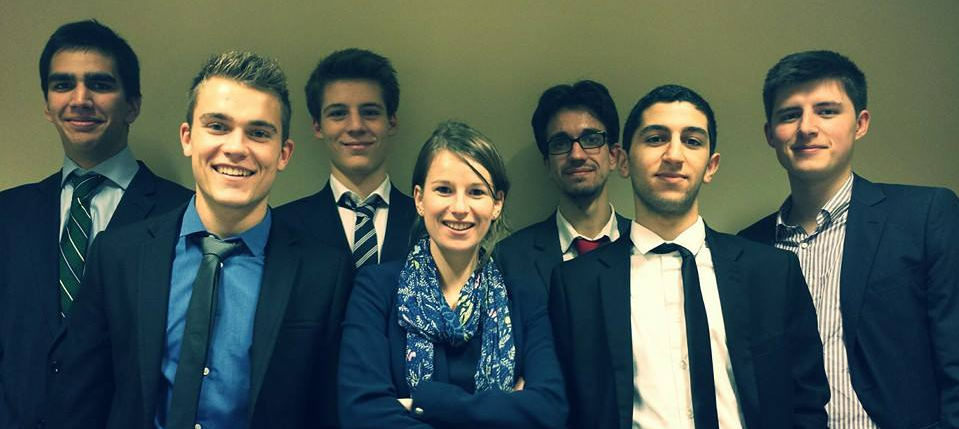
\includegraphics[trim=0cm 0cm 0cm 0cm, clip, width=15cm]{Shema/couverture2.png}
\end{center}
\HRule \\[0.2cm]
%inventer un petit texte cool :)
Dans le cadre de notre projet Q3, il nous a été demandé d'analyser et de proposer des pistes d'amélioration pour le procédé Haber-Bosch. En effet, la synthèse d'ammoniac rejette énormément de \ce{CO2}, c'est pourquoi nous avons exploré des solutions plus écologiques telles que le biométhane, l'hydrolyse ou encore des algues produisant de l'\ce{H2}.
\HRule \\[0.2cm]

\begin{minipage}{0.4\textwidth}
\begin{flushleft} \large
\emph{Auteurs:}
Groupe 1254\\ Simon \bsc{Boigelot} \\ Virgile \bsc{Goyens} \\ Corentin \bsc{Joachim} \\ Xavier \bsc{Lambein} \\Edward \bsc{Nicol}\\ Léa \bsc{Paulus}\\ Abbas \bsc{Sliti}
\end{flushleft}
\end{minipage}
\begin{minipage}{0.4\textwidth}
\begin{flushright} \large
\emph{Cours:} \\
FSAB1503\\
\emph{Groupe:} \\
1254\\
\emph{Tuteur:} \\
Vincent Destoop \textsc{}
\end{flushright}
\end{minipage}
\vspace{0.4cm}
% Bottom of the page

\begin{minipage}{0.3\textwidth}
\begin{flushleft}

\includegraphics[height=2cm]{Shema/logo_UCL_NEW_janv2013.JPG}
\end{flushleft}
\end{minipage}
\begin{minipage}{0.3\textwidth}
\begin{center}
{\large FSA12BA}\\
{\large \today}
\end{center}
\end{minipage}
\begin{minipage}{0.3\textwidth}
\begin{flushright}

\includegraphics[height=1cm]{Shema/epl-logo.jpg}
\end{flushright}
\end{minipage}
\end{center}
\end{titlepage}
\tableofcontents

\documentclass[a4paper,12pt, oneside]{article}

\usepackage[in]{fullpage}

\usepackage[utf8]{inputenc}
\usepackage[T1]{fontenc}
\usepackage[french]{babel}

\usepackage{amsmath}
\usepackage{amssymb}
\usepackage{mathtools}
\usepackage[inline]{enumitem}
\usepackage[squaren,Gray]{SIunits}
\usepackage{sistyle}
\usepackage[autolanguage]{numprint}
\usepackage{xfrac}
\usepackage{bm}
\usepackage{color}
\usepackage[version=3]{mhchem}
\usepackage{multirow}
\usepackage{tabulary}

\newcommand{\diff}[1]{\mathrm{d}#1}

\let\oldvec\vec
\renewcommand{\vec}[1]{\oldvec{\bm{#1}}}
\newcommand{\uvec}[1]{\hat{\bm{#1}}}

\newcommand{\TODO}[1]{\colorbox{red}{\textbf{\textsc{TODO: #1}}}}

\newcommand{\e}[1]{\ensuremath{\cdot 10^{#1}}}

\makeatletter
\newcommand\reaction@[1]{\begin{equation}\ce{#1}\end{equation}}
\newcommand\reaction@nonumber[1]%
{\begin{equation*}\ce{#1}\end{equation*}}
\newcommand\reaction{\@ifstar{\reaction@nonumber}{\reaction@}}
\makeatother


%opening
\title{Rapport 1 : tâche 1}
\author{Groupe 1254}
\date{01-10-2014}

\begin{document}

\maketitle

\tableofcontents

\section{Introduction}




\section{Bilan de masse du plant}

On cherche à calculer les quantités de \ce{CH4}, \ce{H2O} et d'air\footnotemark (respectivement $n_i(\ce{CH4})$, $n_i(\ce{H2O})$ et $n_i(\text{air})$, en moles) nécessaires pour produire $n_f(\ce{NH3})$\;\mole{} d'ammoniac, avec une température du réformeur primaire de $T$\;\kelvin{}.
\footnotetext{La composition de l'air étant : $78\%$ \ce{N2}, $21\%$ \ce{O2}, $1\%$ \ce{Ar}, en fraction molaire.}

Pour ce faire, nous décomposons le bilan en deux parties : tout d'abord, nous allons considérer les réactions se passant au sein du plant (réformeur primaire, réformeur secondaire, WGS et réacteur) et en déduire les quantités de matière nécessaires ; ensuite, nous ajouterons à ce premier bilan la masse de méthane utilisée pour chauffer les réactifs à la température $T$ du réformeur primaire.


\subsection{Bilan des réactions de synthèse}

Pour obtenir ce bilan de masse, nous devons résoudre les dépendances entre les entrées et sorties d'espèces, et les réactions qui se produisent entre ces espèces. Ces dépendances sont de deux types : linéaires --- les réactions chimiques --- et non linéaires --- les constantes d'équilibre thermodynamiques.

\subsubsection{Équations linéaires}

Nous allons commencer par résoudre les relations linéaires. L'ensemble des entrées, sorties et réactions se décomposent de la manière suivante :
\begin{itemize}
  \item entrée de \ce{CH4} et \ce{H2O} ($n_i(\ce{CH4})$ et $n_i(\ce{H2O})$) ;
  \item réformeur primaire (réactions $R_1$ et $R_2$, incomplètes) ;
  \item entrée d'air ($n_i(\text{air})$) ;
  \item réformeur secondaire (réaction $R_3$, complète) ;
  \item water-gas shift (réaction $R_4$, complète) ;
  \item sortie de \ce{H2O} et \ce{CO2} ($n_f(\ce{H2O})$ et $n_f(\ce{CO2})$) ;
  \item synthèse de l'ammoniac (réaction $R_5$, complète) ;
  \item sortie de \ce{Ar} et \ce{NH3} ($n_f(\ce{Ar})$ et $n_f(\ce{NH3})$).
\end{itemize}
Au total, nous avons 12 variables : 3 entrées, 4 sorties et 5 réactions.

La conservation de la masse implique que la somme des entrées, sorties et réactions pour chaque réactif soit égale à zéro. Par exemple, pour \ce{H2O}, cela revient à :
\[
  n_i(\ce{H2O}) - n_f(\ce{H2O}) - R_1 - R_2 - R_4 = 0
\]
Si l'on fait la même chose pour chacune des 9 espèces impliquées, on obtient un système de 9 équations linéaires homogènes à 12 inconnues. La résolution de ce système --- sous forme matricielle, via matlab --- nous donne un espace vectoriel $V$ de dimension 3, qui prend en compte toutes les dépendances linéaires entre les entrées, sorties et réactions.

Pour obtenir une solution unique, il faut donc fournir trois équations supplémentaires pour réduire cet espace à un point. Une de ces équations est linéaire : il s'agit simplement d'égaler $n_f(\ce{NH3})$ au nombre de moles de \ce{NH3} que l'on veut produire.

\subsubsection{Équations non-linéaires}

Les deux dernières équations, comme nous l'avons dit, sont non-linéaires et correspondent aux équilibres thermodynamiques des espèces en présence dans le réformeur primaire (réactions $R_1$ et $R_2$).

À chacune des deux réactions chimiques concernées correspond un quotient réactionnel et une constante d'équilibre, ici $K_1$ et $K_2$. Le calcul détaillé de la valeur ces constantes est \TODO{} fourni en annexe.

À l'aide d'un tableau d'avancement des réactions, nous allons déterminer la quantité de réactifs et de produits au début et à l'équilibre des réactions 1 et 2 :
\begin{center}
  \begin{tabular}{lcccc}
    &  \ce{CH4} & \ce{H2O} & \ce{CO} & \ce{H2}  \\
    \hline
    $n_\text{init}$
    & $n_i(\ce{CH4})$ & $n_i(\ce{H2O})$ & 0 & 0  \\
    $n_\text{eq}$
    & $n_i(\ce{CH4})-R_1$ & $n_i(\ce{H2O})-R_1$ & $R_1$ & $3R_1$
  \end{tabular}
\end{center}
\begin{center}
  \begin{tabular}{lcccc}
    &  \ce{CO} & \ce{H2O} & \ce{CO2} & \ce{H2}  \\
    \hline
    $n_\text{init}$
    & $R_1$ & $n_i(\ce{H2O}) - R_1$ & 0 & 0  \\
    $n_\text{eq}$
    & $R_1-R_2$ & $n_i(\ce{H2O})-R_1-R_2$ & $R_2$ & $R_2$
  \end{tabular}
\end{center}
On voit ici que $R_1$ et $R_2$ symbolisent le degré d'avancement des réactions du réformeur primaire.
%
Les valeurs obtenues dans les deux tableaux d'avancement nous permettent de calculer l'expression des activités des 5 différentes espèces en présence. Soit le gaz $\ce{X}$ et $p_\ce{X}$ sa pression partielle ; son activité est la suivante :
\[
  a_\ce{X} = \frac{p_\ce{X}}{p_\text{tot}} = \frac{n_\ce{X}}{n_\text{tot}} \frac{p_\text{tot}}{p^0}
  \text,
\]
avec $p_\text{tot}$ la pression moyenne du réacteur qui vaut \unit{29}{bar}\footnotemark, $n_\ce{X}$ le nombre de moles de \ce{X} en présence, $n_\text{tot}$ le nombre de moles total en présence --- ici $n_i(\ce{CH4}) + n_i(\ce{H2O}) + 2R_1$ --- et $p^0$ la pression de référence qui vaut \unit{1}{bar}.
\footnotetext{Information trouvée sur le forum du projet.}

À partir de cela, on obtient les équations suivantes :
\begin{align*}
K_1=\frac{a_\ce{CO}(a_\ce{H2})^3}{a_\ce{CH4}a_\ce{H2O}}&=\frac{(R_1-R_2)(3R_1+R_2)^3}{(n_i(\ce{CH4})-R_1)(n_i(\ce{H2O})-R_1-R_2)}
\left(\frac{p_\text{tot}}{(n_i(\ce{CH4}) + n_i(\ce{H2O}) + 2R_1) p^0}\right)^2 \\
K_2=\frac{a_\ce{H2}a_\ce{CO2}}{a_\ce{CO}a_\ce{H2O}}&=\frac{(3R_1+R_2)(R_2)}{(R_1-R_2)(n_i(\ce{H2O})-R_1-R_2)}
\end{align*}

Enfin, l'ajout de ces deux dernières équations à notre système et leur résolution\footnotemark{} réduit à zéro la dimension de l'espace $V$, fournissant la solution au problème, c'est-à-dire la valeur des différents fluxs d'entrée et de sortie, ainsi que les coefficients des réactions.
\footnotetext{Si les équations linéaires étaient encore relativement facile à résoudre à la main, les équations que nous avons ici sont d'un degré bien trop élevé et nécessitent un outil numérique --- dans notre cas Matlab.}



% Dans l'ordre, les colonnes sont : $n_i(\ce{CH4})$, $n_i(\ce{H2O})$, $n_i(\text{air})$, $n_f(\ce{H2O})$, $n_f(\ce{CO2})$, $n_f(\ce{Ar})$, $n_f(\ce{NH3})$, $R_1$, $R_2$, $R_3$, $R_4$ et $R_5$.
% \[
% \left(
% \begin{array}{*{12}c}
%   1 & 0 & 0 & 0 & 0 & 0 & 0 & -1 & 0 & -2 & 0 & 0 \\
%   0 & 1 & 0 & -1 & 0 & 0 & 0 & -1 & -1 & 0 & -1 & 0 \\
%   0 & 0 & 0 & 0 & 0 & 0 & 0 & 3 & 1 & 4 & 1 & -3 \\
%   0 & 0 & 0 & 0 & 0 & 0 & 0 & 1 & -1 & 2 & -1 & 0 \\
%   0 & 0 & 0 & 0 & -1 & 0 & 0 & 0 & 1 & 0 & 1 & 0 \\
%   0 & 0 & .21 & 0 & 0 & 0 & 0 & 0 & 0 & -1 & 0 & 0 \\
%   0 & 0 & .78 & 0 & 0 & 0 & 0 & 0 & 0 & 0 & 0 & -1 \\
%   0 & 0 & .01 & 0 & 0 & -1 & 0 & 0 & 0 & 0 & 0 & 0 \\
%   0 & 0 & 0 & 0 & 0 & 0 & -1 & 0 & 0 & 0 & 0 & 2
% \end{array}
% \right)
% \]


\subsection{Bilan de la combustion du méthane}



\subsection{Bilan total}


\section{Nombre de tuyaux d'alimentation}

Grâce au programme Matlab que nous avons écrit, nous sommes arrivés à déterminer le nombre de moles journalières de \ce{CH4} nécessaires pour pouvoir produire 1500 tonnes d'ammoniac par jour. A partir de cela, nous sommes parvenus à exprimer le débit de masse du \ce{CH4} qui est:
    $$\dot{m}=\frac{m_{\ce{CH4}}}{\unit{24}{\hour}}$$
    $$\dot{m}=\frac{\unit{625.9}{\ton}}{\unit{86400}{\second}}=\unit{7.24}{\kilogram\per\second}$$

On cherche dans un premier temps le flux d'écoulement de \ce{CH4}, $\dot{V}_{tot}$. On sait que :
$\dot{V}_{tot}={\dot{m}}/{\rho}$.
Il nous faut donc $\dot{m}$ (connu) et $\rho$. On sait aussi que:
\[ \rho = \frac{1}{v} \]
Selon la loi des gaz parfaits:
\begin{align*}
    pv &= R^{*}T \quad\Leftrightarrow\quad v = \frac{R\cdot T}{M\cdot p} \\
    v &= \frac{\unit{8.314}{\joule\per\kelvin\mole}\cdot\unit{1080}{\kelvin}}{\unit{16\cdot10^{-3}}{\kilogram\per\mole}\cdot\unit{31}{bar}}=\unit{0.18}{\cubic\meter\per\kilogram}
\end{align*}
Et donc:
\[
    \rho = \frac{1}{v} = \unit{5.52}{\kilogram\per\cubic\meter}
    \qquad\text{et}\qquad
    \dot{V}_{tot} = \frac{\dot{m}}{\rho}=\unit{1.31}{\cubic\meter\per\second}
\]

Pour trouver le nombre de tuyaux nécessaires, il nous faut diviser $\dot{V}_{tot}$ par le débit d'un seul tuyau $\dot{V}_{1t} = A\cdot c = \pi r^2 c$. Connaissant le rayon d'un tuyau ($r=\unit{0.05}{\meter}$) et la vitesse ($c=\unit{2}{\meter\per\second}$), on a :
\[
    x = \frac{\dot{V}_{tot}}{\dot{V}_{1t}}
      = \frac{\unit{1.31}{\cubic\meter\per\second}}{\unit{0.0157}{\cubic\meter\per\second}}
      = \unit{83.39}{tuyaux}
\]

Il nous faudrait donc 84 tuyaux pour satisfaire le besoin en \ce{CH4} dans le réacteur du reformage primaire.

Parallèlement, connaissant la masse d'eau demandée par le réformeur primaire grâce à notre programme Matlab (\unit{1386.79}{\ton}) et en utilisant un raisonnement analogue au précédent, on obtient que le nombre de tuyaux nécessaire pour le transport de l'eau est de 151.

Au total, nous aurons donc besoin de 229 tuyaux pour approvisionner notre réformeur primaire à la fois en \ce{CH4} et en eau.


\begin{appendices}

\newpage
\section{Flowsheet}\label{appendix:flowsheet}

\tikzstyle{decision} = [diamond, draw, fill=blue!20,
    text width=4.5em, text badly centered, node distance=3cm, inner sep=0pt]
\tikzstyle{block} = [rectangle, draw, fill=blue!20,
    text width=14em, text centered, rounded corners, minimum height=4em, minimum width=15em, node distance=3cm]
\tikzstyle{block2} = [rectangle, draw, fill=red!20,
    text width=14em, text centered, rounded corners, minimum height=4em, minimum width=15em, node distance=3cm]
\tikzstyle{line} = [draw, -latex']
\tikzstyle{cloud} = [draw, ellipse,fill=red!20, node distance=3cm,
    minimum height=2em]

\begin{center}
	%\begin{tikzpicture}[thick,scale=0.6, every node/.style={scale=0.6}]
	\begin{tikzpicture}[node distance = 3cm, auto]
	    % Place nodes
	    \node [block] (RefPrim) {\textbf{Réformage primaire}(Réformage à vapeur de \ce{CH_4}) $$\ce{CH_4 + H_2O <=> CO + 3H_2}$$ $$\ce{CO + H2O <=> H2 + CO2}$$ \textit{Equilibre à T (sortie)} };
	    \node [block2, left of=RefPrim, node distance=7cm] (Four) {\textbf{Four} \\ Combustion de \ce{CH_4} \\ \textit{Irreversible et complète}};
	    \node [block, below of=RefPrim, node distance=3.5cm] (RefSec) {\textbf{Réformage secondaire} $$\ce{2CH4 + O2 -> 2CO + 4H2}$$ \textit{Considérée comme irréversible et complète à la fin.}};
	    \node [block, below of=RefSec, node distance=3.5cm] (Reacteur) {\textbf{Réacteurs Water-Gas-Shift} $$\ce{CO + H2O -> CO2 + H2}$$ \textit{Considérée comme complète à la fin.} };
	    \node [block, below of=Reacteur, node distance=3.5cm] (AbsComp) {\textbf{Absorption de \ce{CO2} et compression} (séparation d'\ce{H2 O}) \\ \textit{Considérées complètes.}};
	    \node [block, below of=AbsComp, node distance=3.5cm] (Synth) {\textbf{Synthèse d'\ce{NH3} et séparation} $$\ce{N2 + 3H2 <=> 2NH3}$$ \textit{Considérées complètes.}};
	    \node [right of =AbsComp, node distance=6cm] (nothing1){};
	    \node [below of =Synth] (nothing2){};
	    \node [left of =RefSec, node distance=6cm] (nothing3){};
	    \node [above of =RefPrim, node distance=4cm] (nothing4){};
	    \node [left of =Four, node distance=5cm] (nothing5){};
	    \node [above of =Four, node distance=4cm] (nothing6){};
	    % Draw edges
	    \path [line] (RefPrim) -- node {\ce{CH4}, \ce{H2O}}(RefSec);
	    \path [line] (Four) -- node {ENERGY} (RefPrim);
	    \path [line] (RefSec) -- (Reacteur);
	    \path [line] (Reacteur) -- node {\ce{CO2(g) + H2(g)}} (AbsComp);
	    \path [line] (AbsComp) -- (Synth);
	    \path [line] (AbsComp) -- node {\ce{CO2(g)}, \ce{H2O(g)}}(nothing1);
	    \path [line] (Synth) -- node {\ce{NH3(l)}, \ce{Ar(g)}}(nothing2);
	    \path [line] (nothing3) -- node {\ce{O2(g)}, \ce{N2(g)},\ce{Ar(g)}}(RefSec);
	    \path [line] (nothing4) -- node {\ce{CH4(g)}, \ce{H2 O(l)}}(RefPrim);
	    \path [line] (Four) -- node {\ce{CO2+2H2O}} (nothing5);
	    \path [line] (nothing6) -- node {\ce{CH4(g), H2O(l)}} (Four);
	\end{tikzpicture}
\end{center}


\section{Système linéaire du bilan de masse}\label{appendix:matrix}

Pour éventuellement aider à comprendre le fonctionnement du bilan de masse, nous fournissons ici le système, sous forme matriciel, qui est à résoudre pour obtenir l'espace vectoriel $V$.

Dans l'ordre, les lignes de la matrice correspondent aux composés suivants : \ce{CH4}, \ce{H2O}, \ce{O2}, \ce{N2}, \ce{Ar}, \ce{CO},  \ce{CO2}, \ce{H2} et \ce{NH3}.
\[
\left(
\begin{array}{*{12}c}
  1 & 0 & 0 & 0 & 0 & 0 & 0 & -1 & 0 & -2 & 0 & 0 \\
  0 & 1 & 0 & -1 & 0 & 0 & 0 & -1 & -1 & 0 & -1 & 0 \\
  0 & 0 & 0 & 0 & 0 & 0 & 0 & 3 & 1 & 4 & 1 & -3 \\
  0 & 0 & 0 & 0 & 0 & 0 & 0 & 1 & -1 & 2 & -1 & 0 \\
  0 & 0 & 0 & 0 & -1 & 0 & 0 & 0 & 1 & 0 & 1 & 0 \\
  0 & 0 & .21 & 0 & 0 & 0 & 0 & 0 & 0 & -1 & 0 & 0 \\
  0 & 0 & .78 & 0 & 0 & 0 & 0 & 0 & 0 & 0 & 0 & -1 \\
  0 & 0 & .01 & 0 & 0 & -1 & 0 & 0 & 0 & 0 & 0 & 0 \\
  0 & 0 & 0 & 0 & 0 & 0 & -1 & 0 & 0 & 0 & 0 & 2
\end{array}
\right)
\left(
\begin{array}{*{1}c}
  n_{i,\ce{CH4}} \\ n_{i,\ce{H2O}} \\ n_{i,\text{air}} \\ n_{f,\ce{H2O}} \\ n_{f,\ce{CO2}} \\ n_{f,\ce{Ar}} \\ n_{f,\ce{NH3}} \\ R_1 \\ R_2 \\ R_3 \\ R_4 \\ R_5
\end{array}
\right)
= 0
\]


%\section{Calcul des constantes d'équilibre}\label{appendix:const_eq}

Nous avons calculé les constantes d'équilibre des réactions 1 et 2 avec Matlab, à l'aide de l'expression suivante :
\[
    K = \mathrm{exp}\!\left( -\frac{\Delta G^0_m(T)}{RT} \right)
      = \mathrm{exp}\!\left( \frac{\Delta S^0_m(T)}{R} - \frac{\Delta H^0_m(T)}{RT} \right)
    \text.
\]
Dans cette expression, le symbole $\Delta$ correspond à la différence entre les produits et les réactifs. Par exemple, $\Delta S^0_m(T)$ est la somme de l'entropie molaire des produits moins l'entropie molaire des réactifs.

Il est donc nécessaire d'obtenir $\Delta S^0_m(T)$ et $\Delta H^0_m(T)$. Ceux-ci sont calculés à l'aide des formules :
\[
    \Delta S^0_m(T) = \Delta S^0_m(T_0) + \int_{T_0}^T\! \Delta C_{p,m} \frac{\diff{T}}{T}
    \qquad\text{et}\qquad
    \Delta H^0_m(T) = \Delta H^0_m(T_0) + \int_{T_0}^T\! \Delta C_{p,m} \diff{T}
    \text.
\]
Enfin, la différence de capacités calorifiques molaires $\Delta C_{p,m}$ qui apparait ici est obtenue, sous forme de polynomes de $T$, dans des tables thermodynamiques. Il en va de même pour l'enthalpie et l'entropie à la température de référence $T_0$.

Nous avons donc tous les outils nécessaires pour calculer la valeur de $K$ dans les deux réactions du réformeur primaire. Il suffit simplement d'implémenter les formules dans Matlab pour obtenir les constantes d'équilibres utilisées dans le calcul du bilan de masse.


\end{appendices}

\end{document}

\documentclass[10pt,a4paper]{article}

\usepackage[in]{fullpage}

\usepackage[utf8]{inputenc}
\usepackage[T1]{fontenc}
\usepackage[french]{babel}

\usepackage{amsmath}
\usepackage{amssymb}
\usepackage{mathtools}
\usepackage[inline]{enumitem}
\usepackage[squaren,Gray]{SIunits}
\usepackage{sistyle}
\usepackage[autolanguage]{numprint}
\usepackage{xfrac}
\usepackage{bm}
\usepackage{color}
\usepackage[version=3]{mhchem}
\usepackage{multirow}
\usepackage{tabulary}

\newcommand{\diff}[1]{\mathrm{d}#1}

\let\oldvec\vec
\renewcommand{\vec}[1]{\oldvec{\bm{#1}}}
\newcommand{\uvec}[1]{\hat{\bm{#1}}}

\newcommand{\TODO}[1]{\colorbox{red}{\textbf{\textsc{TODO: #1}}}}

\newcommand{\e}[1]{\ensuremath{\cdot 10^{#1}}}

\makeatletter
\newcommand\reaction@[1]{\begin{equation}\ce{#1}\end{equation}}
\newcommand\reaction@nonumber[1]%
{\begin{equation*}\ce{#1}\end{equation*}}
\newcommand\reaction{\@ifstar{\reaction@nonumber}{\reaction@}}
\makeatother


\begin{document}

\section{Synthèse \ce{NH3} et séparation}

Nous allons maintenant étudier de manière plus précise la dernière étape du procédé qui comprend le réacteur de synthèse d’ammoniac et l'étape de séparation des produits.
La réaction de synthèse de \ce{NH3} est suivante :
\[ \ce{N_2 + 3H2 <=> 2NH3} \]

\subsection{Manière qualitative}

Voyons de quelle manière évolue la réaction en faisant varier d'une part la température, et d'autre part la pression. Pour cela, nous nous basons sur le fait qu'une réaction chimique a toujours tendance à   aller à l'encontre des modifications qui lui sont apportées, à savoir le principe énoncé par le Chatelier. Dans notre cas, nous devons favoriser la réaction allant dans le sens de production de \ce{NH3}.

Tout d'abord, regardons ce qu'il en est au niveau de la pression. Nous devons augmenter celle-ci car de cette manière le système réagira en favorisant le sens de réaction produisant un plus petit nombre de moles de gaz, à savoir \ce{NH3} dans le but de rétablir la pression. 

Ensuite, nous allons étudier le comportement de notre réaction lorsqu'on modifie la température. Pour cela, nous devons déterminer si la réaction est endothermique ou exothermique. Nous calculons donc le $\Delta H$  de la réaction.
\[ \Delta H^0_r = \unit{-92,4}{\kilo\joule\per\mole} \]
Le signe de $\Delta H$ étant négatif, notre réaction est bien exothermique. De ce fait, nous devons diminuer la température afin de favoriser la réaction à libérer de la chaleur, et donc de favoriser les produits.

Nous en venons donc à la conclusion qu'il nous faudrait une pression théoriquement infinie et une température la plus basse possible. Cependant, nous sommes restreint économiquement et techniquement, nous devons donc trouver un juste milieu, une conversion totale n'est donc pas envisageable. 
\\

Une pression très élevée est économiquement et techniquement irréalisable car les tuyaux et autres équipements supportant les flux devront aligner leurs performances pour répondre à des critères beaucoup plus stricts qu'avec de basses pressions.
Pour cette raison, il serait plus judicieux de réinjecter  le diazote et le dihydrogène qui n'ont pas réagi au cours de la réaction (la réaction est à l'équilibre!) dans le réacteur. Pour effectuer cette séparation, les éléments du réacteur sont refroidis, l'ammoniac est liquéfié (l'ammoniac se condense à température plus élevé que le dihydrogène et diazote) et les réactifs sont réintroduits dans le réacteur.

\subsection{Manière quantitative}

De manière plus rigoureuse, nous pouvons démontrez l'influence de la température et de la pression de notre réaction à l'aide d'une modélisation mathématique.

Démontrons qu'une diminution de la température favorise la production de produits pour toute réaction exothermique avec l'équation de Van't Hoff.
\[ \ln{\frac{K_2}{K_1}} = \frac{\Delta H^0_r}{R} \left(\frac{1}{T_1} - \frac{1}{T_2}\right) \]

$ \Delta H^0_r < 0$, si $T_2<T_1$ alors $1/T_2 > 1/T_1$. Donc $\ln{K_2/K_1} > 0$, ce qui implique que $K_2/K_1>1$  et donc que $ K_2>K_1$.

Si $K$ augmente la réaction favorise les produits, le principe de Le Chatelier est donc bien vérifié pour la température.
\\

Pour la pression, il faut étudier l'influence de la pression totale $p_{tot}$ dans le quotient réactionnel $Q_r$ car $K(T)$ ne dépend que de la température. Ensuite, il suffit de comparer $Q_r$ et  $K(T)$ sans faire varier la température. 
\[ Q_r= \frac{{(\chi_\ce{NH3} p_{tot})}^2}{(\chi_\ce{N2} p_{tot}) \cdot {(\chi_\ce{H2} p_{tot})}^3}=\frac{{\chi_\ce{NH3}}^2}{\chi_\ce{N2} {\chi_\ce{H2}}^3 \textcolor{red}{{p_{tot}}^2}} \]

Lorsque la pression augmente, $Q_r$ diminue, $Q_r < K$ et donc la réaction favorise les produits.
 
Lorsque la pression diminue, $Q_r$ augmente, $Q_r > K$ et donc la réaction favorise les réactifs.

Le principe de Le Chatelier est vérifié pour la pression.

\end{document}

\documentclass[a4paper,12pt, oneside]{article}

\usepackage[in]{fullpage}

\usepackage[utf8]{inputenc}
\usepackage[T1]{fontenc}
\usepackage[french]{babel}

\usepackage{amsmath}
\usepackage{amssymb}
\usepackage{mathtools}
\usepackage[inline]{enumitem}
\usepackage[squaren,Gray]{SIunits}
\usepackage{sistyle}
\usepackage[autolanguage]{numprint}
\usepackage{xfrac}
\usepackage{bm}
\usepackage{color}
\usepackage[version=3]{mhchem}
\usepackage{multirow}
\usepackage{tabulary}

\newcommand{\diff}[1]{\mathrm{d}#1}

\let\oldvec\vec
\renewcommand{\vec}[1]{\oldvec{\bm{#1}}}
\newcommand{\uvec}[1]{\hat{\bm{#1}}}

\newcommand{\TODO}[1]{\colorbox{red}{\textbf{\textsc{TODO: #1}}}}

\newcommand{\e}[1]{\ensuremath{\cdot 10^{#1}}}

\makeatletter
\newcommand\reaction@[1]{\begin{equation}\ce{#1}\end{equation}}
\newcommand\reaction@nonumber[1]%
{\begin{equation*}\ce{#1}\end{equation*}}
\newcommand\reaction{\@ifstar{\reaction@nonumber}{\reaction@}}
\makeatother

\title{Tâche 4 : Mini-Hazop}
\author{Groupe 1254}
\begin{document}
\maketitle
\section{Dangers des substances}
Premièrement, on retrouve dans la production d'ammoniac deux réactifs sous forme de gaz: l'azote, \ce{N2}, et l'hydrogène, \ce{H2}. Ces gaz ont la particularité d'être à la fois incolores et inodores. Le premier présente un danger de par le fait qu'il va "prendre la place" de l'oxygène présent dans l'air, provoquant ainsi un risque d'asphyxie (un taux d'oxygène inférieur à 19\% est létal). 
		
		L'hydrogène quant à lui est d'une part explosif (une fuite d'hydrogène augmentant donc grandement le risque d'incendies!) et d'autre part fortement corrosif envers les couches de fer composant les parois des réacteurs et reformeurs. Ainsi, ce composé crée des lèvres et des fissures dans lesdites parois, provoquant l'échappement des gaz présents dans le procédé chimique.
		
		En second lieu, l'ammoniac qui est lui aussi sous forme gazeuse, implique bien des risques. Bien qu'il soit facilement repérable grâce à son odeur particulière et prononcée (odeur repérable à partir de 5 ppm), il représente de gros risques pour la santé. En effet, une concentration d'\ce{NH3} comprise entre 400 et 700 ppm provoquera chez un inhalateur des irritations de la gorge variant en intensité tandis qu'une concentration de 10 000 ppm provoquera de graves conséquences médicales.

		Par ailleurs, l'ammoniac peut devenir explosif sous certaines conditions particulières de température et de pression. Il attaque également le zinc et le cuivre, nécessitant un équipement approprié lors de sa manipulation. Finalement, le \ce{NH3} présent sous l'état liquide s'évapore très rapidement lorsqu'il entre en contact avec de l'eau: il faudra donc pratiquer le spinning si nous sommes amenés à nettoyer une  flaque d'ammoniac.

\section{Circulation des flux de matière}

\begin{figure}
	\includegraphics[scale=0.6]{Plan1.png}
	\caption{Circulation du flux}
	\label{cir1}
	\end{figure}
\begin{figure}
	\includegraphics[scale=0.5]{Plan2.png}
	\caption{Circulation du flux}
	\label{cir2}
\end{figure}
\begin{figure}
	\includegraphics[scale=0.5]{Plan2-2.png}
	\caption{Circulation du flux}
	\label{cir3}
	\end{figure}
\begin{figure}
\includegraphics[scale=0.4]{Position_des_differents_noeuds.png} 
	\caption{Position des  Noeuds}
	\label{cir4}
\end{figure}
Les flux et noeuds se trouvent aux figures~\ref{cir1},\ref{cir2},\ref{cir3}.
Le positionnement des noeuds se trouve à la figure~\ref{cir4}.

\section{Tableau de la mini-HAZOP}

(voir tableau excel)

\section{Soupape}
La réaction de production d'ammoniac du procédé que nous utilisons (\bsc{Haber} - \bsc{Bosch}) est la suivante:
$$\ce{N2 +3H2 <=> 2NH3}$$
Cette réaction est donc caractérisée par une diminution de moles de gaz. En nous rappelant la loi des gaz parfaits, on peut déduire que la réaction est aussi caractérisée par une diminution de pression. Il y a donc peu de risque d'une surpression dans le réacteur principal, rendant l'ajout d'une soupape et / ou d'un disque de rupture inutile.

\section{Disque de rupture}
L'eau chauffant, dans l'échangeur 124-MC, nous avons une augmentation de pression car $$pV=nRT$$ et que le nombre de mole reste constant. Cette pression augmentante entraîne alors un danger de suppression, un disque de rupture est alors nécessaire afin d'avoir une installation sécurisée.

\end{document}

\chapter{Dimensionnement d'une soupape de sécurité}

\section{Contexte}
Il nous ait demandé de prévoir une soupape de sécurité à installer sur un tank de \ce{NH_3} à l'état liquide. En effet, ce tank est situé à proximité d'un réservoir de mazout et celui-ci représente un risque d'ignition qui pourrait causer une surpression sur le tank. 

\section{\large{Données:}}
\begin{itemize}
\item Hauteur totale du tank : 12\meter
\item Niveau de \ce{NH_3} liquide dans le tank : 8\meter
\item Diamètre du tank : 6\meter
\item T normale de stockage : 20\celsius
\item Pression de design : 15 barg
\item Cp/Cv du \ce{NH_3} : 1.33
\item Facteur de compressibilité Z : 1.0
\end{itemize}

\section{Questions}
\begin{enumerate}
\item\textit{Quelle est la pression normale de stockage?}

En utilisant le graphe de la pression en fonction de la température donné dans l'énoncé et sachant que la température de stockage est de 20\celsius , nous pouvons aisément en déduire la pression normale de stockage qui sera approximativement de 7.5 barg, soit 8.51325 bar.

\item\textit{Quelle sera la pression de stockage en été (30\celsius)?}

De la même manière, mais en utilisant cette fois une température de stockage de 30\celsius , nous trouvons une pression de 11 barg, soit 12.01325 bar.

\item\textit{Quelle sera la pression maximale de tarage de la soupape de sécurité?}

La pression de tarage maximale d'une soupape doit toujours être supérieure à la pression opératoire mais également inférieure à la pression de design. Supérieure à la pression opératoire afin d'avoir une marge si jamais une petite surpression venait à se produire sans pour autant être dangereuse. Cela nous évite de perdre toute une \og fournée \fg. Inférieure à la pression de design parce que la soupape ne sait pas immédiatement rétablir l'ordre et que la pression continue donc à monter un petit peu avant d'atteindre son maximum. 
Dans notre cas, la pression maximale de tarage sera donc de 15 barg, soit 16.01325 bar 

\item\textit{Quelle sera la pression durant la décharge?}

Dans le cas traité, c'est-à-dire quand l'accident est un incendie, on doit considérer que la décharge se fera à une pression de 121\% de la pression de tarage. Celle-ci étant fixée à 16.01325 bar, la pression lors de la décharge sera donc de 19.376 bar.

\item\textit{Quelle sera la temperature du liquide durant la décharge via la soupape?}

Ayant trouvé la pression de décharge, on peut directement trouver la température à l'aide du graphique. Elle vaut 323.15\kelvin.

\item\textit{Quelle sera la taille de la soupape nécessaire?}
La formule déterminant la chaleur totale absorbée par le liquide est: $$ Q = C \cdot F \cdot A^{0.82} $$
Dans notre cas,
\begin{itemize}
\item C = 43 200
\item F = 1
\item A = 143.2566 \meter\squared
\end{itemize}
Nous trouvons donc une chaleur \unit{2.5322}{\megad\watt}.
Sachant que la pression maximale de tarage est de 15 barg, nous pouvons en déduire la température à l'aide du graphique. Celle-ci est donc de 40\celsius, soit 313.15\kelvin. En utilisant le second graphe, nous trouvons que l'enthalpie de vaporistion vaut \unit{1150}{\kilo\joule\per\kilogram}. Ainsi, nous pouvons obtenir le flux de masse. $$ W = \frac{Q}{\Delta H_{vap}} = \frac{\unit{2.5322}{\megad} \cdot 3600}{\unit{1150}{\kilod}} = \unit{7.9269}{\kilod\kilogram\per\hour} $$
Afin d'obtenir l'aire de l'orifice de la soupape, nous avons utilisé la formule suivante:
$$ A = \frac{W}{C \cdot K_d \cdot P_1 \cdot K_b \cdot K_c}\cdot\sqrt{\frac{T \cdot Z}{M}} $$ avec $$ C = 0.03948\cdot\sqrt{k\cdot\left(\frac{2}{k+1}\right)^\frac{k+1}{k-1}} $$
Ce qui nous donne $ C = 0.0265$ et donc $A = \unit{680}{\microd\meter\squared}$.

L'aire de l'orifice de notre soupape est donc de \unit{680}{\microd\meter\squared}.

\item\textit{Si la pression de design de l'équipement était 20 barg, quel serait l'effet d'augmenter la pression de tarage de 5 bar et de la porter à 20 barg?}

La soupape ne sait pas agir directement dans la seconde. Si on met la pression de tarage à 20 barg, la soupape s'ouvre à cette pression mais la pression continuera à augmenter encore un peu avant d'atteindre son maximum et puis de diminuer. Ce qui fait qu'il est possible d'atteindre une pression plus haute que la pression de design de l'équipement. Celui-ci pourrait donc être endommagé.

\item\textit{Pour la première pression de tarage, quelle est l'influence d'isoler thermiquement le tank tel que le coefficient d'échange avec l'extérieur soit réduit à une valeur de 10 \watt\per\meter\squared\kelvin ?}

En isolant le tank, on diminue le facteur d'environnement. En effet, celui-ci vaudrait alors 0.15. Multiplier la facteur d'environnement par 15\% revient à multiplier la chaleur totale reçue de 15\%, ce qui revient à multiplier de 15\% le flux de masse, ce qui revient à multiplier de 15\% l'aire de l'orifice de la soupape. Nous aurions donc besoin d'une soupape dont l'aire de l'orifice vaut 102 \microd\meter\squared.
\end{enumerate}

\chapter{Activités de terrain}

\section{Production d'hydrogène par électrolyse}

Au cours du laboratoire, nous avons fait varier plusieurs paramètres afin de déterminer les meilleures conditions de production d'hydrogène. Les trois paramètres sont le pH, la température et le courant (en Ampère). Nous avons étudié la vitesse de production d'hydrogène.
\\

Remarque : Certaines mesures manquent ou sont imprécises, nous nous sommes donc inspirées de la solution donnée. \footnote{les graphiques sont tirés du document corrigé fournis sur icampus}

\subsection{Conditions opératoires de production d'hydrogène}

\subsubsection{La température}

La température influence la vitesse de réaction : une augmentation de température implique un apport de chaleur qui contribue à diminuer l'énergie à apporter à la réaction (qui est endothermique) et donc l'énergie électrique à apporter sera moindre.



\subsubsection{Le courant}

\begin{figure}
\begin{center}
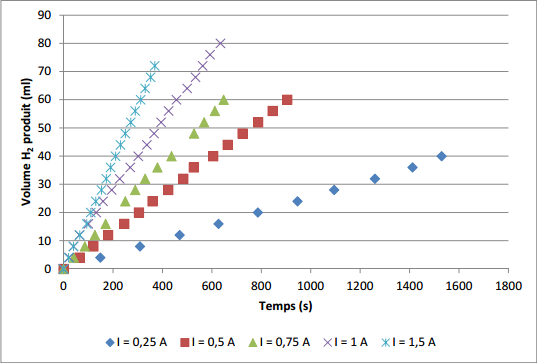
\includegraphics[scale=0.7]{task7/PRODUCTIONHYDRO.png} 
\end{center}
\caption{Effet du courant sur la production d'\ce{H2}}
\label{courant-H2}
\end{figure}

Le courant est un paramètre qui influence directement la vitesse de production d'hydrogène. De plus, ces deux grandeurs sont proportionnelles, la production d'hydrogène est donc linéaire avec le temps. En effet, nous nous sommes aperçus que doubler le courant doublait également la vitesse de production (voir figure \ref{courant-H2}). Cependant, nous verrons que celle-ci peut être perturbée par l'acidité du milieu(pH). Par conséquent, plus le courant est élevé plus le flux d'hydrogène sera important.

\subsubsection{L'acidité du milieu}


\begin{figure}
\begin{center}
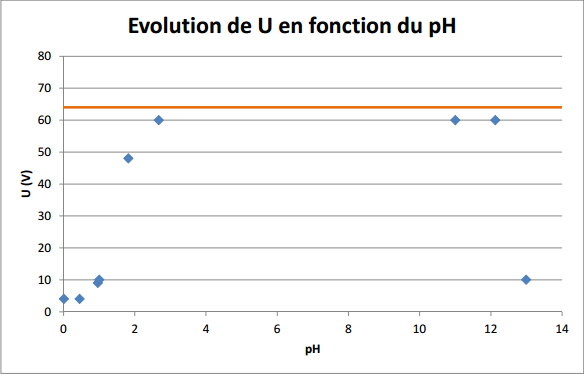
\includegraphics[scale=0.7]{task7/poi.png}
\end{center}
\caption{Evolution de la tension en fonction du pH}
\label{tension-ph}
\end{figure}

La variation du pH peut influencer la vitesse de production de l'hydrogène. Pour obtenir un même courant à des pH différents, il fallait ajuster la tension (V). A certains pH, il était même impossible d'obtenir un courant de \unit{0.5}{A} à cause de la tension limitée que pouvait produire notre générateur (\unit{64}{V} maximum). Il est donc important de bien ajuster l'acidité du milieu en fonction du générateur à disposition. On remarque donc que le pH influence bien la production d'hydrogène car une augmentation de tension implique une augmentation de la puissance (voir figure \ref{tension-ph}). Cependant, l'électrolyse peut se réaliser sans apport de changement de pH. Il est, économiquement, préférable de réaliser cette expérience à pH neutre car le modifier suggère d'importer des réactifs supplémentaires en grande quantité bien qu'il faille imposer une puissance plus intense. 

\subsection{Puissance requise pour un flux d'hydrogène}

Pour produire \unit{1500}{t/j} d'ammoniac, il faut disposer d'un flux d'hydrogène de \unit{1529.1}{mol/s}. Nous supposerons que le rendement est de \unit{100}{\%} et que la réaction se déroule dans les conditions standard. 

La réaction de l’électrolyse de l'eau est la suivante : 
$$\ce {2H2O(l) -> 2H2(g) + O2(g)}$$ 

Calculons l'enthalpie molaire de réaction :

$$ \Delta H_r^0 =  \unit{285}{kJ.mol^{-1}} $$

La puissance (P) à fournir au système est simplement le produit du flux d'hydrogène exigé et de $ \Delta H_r^0$ :

$$ P = 285\cdot1529.1 = \unit{435 793.5}{kW} $$
\section{Visite de Total à Feluy}

Nous avons visité l'entreprise Total située à Feluy, c'est une entreprise pétrolière qui s'occupe de produire et fournir de l'énergie. Notre visite s'est déroulée en différentes étapes, tout d'abord une petite présentation sur l'entreprise elle-même ainsi que sa place dans le marché mondial. Ensuite, nous avons pu visiter différentes parties de l'entreprise ainsi que l'unité pilote qui leur permet de réaliser des tests à plus petite échelle afin de ne pas bloquer l'entiereté de la production en cas de tests défayants.

\subsection{Le rôle des catalyseurs}

Les catalyseurs jouent un rôle essentiel dans une grande partie des réactions chimiques. En effet, ceux-ci permettent d'augmenter la vitesse de la réaction ainsi que son rendement, ce qui est primordial dans la chaîne de production d'une entreprise. Le catalyseur va affaiblir la molécule qui réagit, ce qui va permettre à la réaction de se dérouler plus rapidement.
On place souvent ces catalyseurs sur un support poreux ce qui a pour effet de sélectionner uniquement certaines molécules. Les catalyseurs sont également très utiles pour diriger une réaction lorsque qu'un réactif peut réagir de diverses manières, cela permet de diminuer les pertes vers d'autres réactions. Cependant, il faut savoir qu'il existe des réactions où le catalyseur est indispensable, sans lui rien ne se passe.

\subsection{Sécurité}

Dans une entreprise de telle ampleur, il est indispensable d'avoir des mesures de sécurité à respecter pour la santé de la population ainsi que du point de vue environnemental. Il existe donc une multitude de précautions à prendre. Sur le site de Feluy, nous avons, par exemple, remarqué ces tours qui montent à une centaine de mètres de hauteur, elles permettent en cas de problèmes, de brûler les composants et de les faire sortir vers l'exterieur. La hauteur se justifie par la quantité de chaleur qui est dégagée lors de ce processus.

\documentclass[a4paper,12pt, oneside]{article}

\usepackage[in]{fullpage}

\usepackage[utf8]{inputenc}
\usepackage[T1]{fontenc}
\usepackage[french]{babel}

\usepackage{amsmath}
\usepackage{amssymb}
\usepackage{mathtools}
\usepackage[inline]{enumitem}
\usepackage[squaren,Gray]{SIunits}
\usepackage{sistyle}
\usepackage[autolanguage]{numprint}
\usepackage{xfrac}
\usepackage{bm}
\usepackage{color}
\usepackage[version=3]{mhchem}
\usepackage{multirow}
\usepackage{tabulary}

\newcommand{\diff}[1]{\mathrm{d}#1}

\let\oldvec\vec
\renewcommand{\vec}[1]{\oldvec{\bm{#1}}}
\newcommand{\uvec}[1]{\hat{\bm{#1}}}

\newcommand{\TODO}[1]{\colorbox{red}{\textbf{\textsc{TODO: #1}}}}

\newcommand{\e}[1]{\ensuremath{\cdot 10^{#1}}}

\makeatletter
\newcommand\reaction@[1]{\begin{equation}\ce{#1}\end{equation}}
\newcommand\reaction@nonumber[1]%
{\begin{equation*}\ce{#1}\end{equation*}}
\newcommand\reaction{\@ifstar{\reaction@nonumber}{\reaction@}}
\makeatother



\begin{document}

\chapter{Activité de terrain: visite de Yara à Tertre}
\section{Sécurité}
	\subsection{Risques encourus}
		Premièrement, on retrouve dans la production d'ammoniac deux réactifs sous forme de gaz: l'azote, \ce{N2}, et l'hydrogène, \ce{H2}. Ces gaz ont la particularité d'être à la fois incolores et inodores. Le premier présente un danger de par le fait qu'il va "prendre la place" de l'oxygène présent dans l'air, provoquant ainsi un risque d'asphyxie (un taux d'oxygène inférieur à 19\% est létal). 
		
		L'hydrogène quant à lui est d'une part explosif (une fuite d'hydrogène augmentant donc grandement le risque d'incendies!) et d'autre part fortement corrosif envers les couches de fer composant les parois des réacteurs et reformeurs. Ainsi, ce composé crée des lèvres et des fissures dans lesdites parois, provoquant l'échappement des gaz présents dans le procédé chimique.
		
		En second lieu, l'ammoniac qui est lui aussi sous forme gazeuse, implique bien des risques. Bien qu'il soit facilement repérable grâce à son odeur particulière et prononcée (odeur repérable à partir de 5 ppm), il représente de gros risques pour la santé. En effet, une concentration d'\ce{NH3} comprise entre 400 et 700 ppm provoquera chez un inhalateur des irritations de la gorge variant en intensité tandis qu'une concentration de 10 000 ppm provoquera de graves conséquences médicales.
		
		Par ailleurs, l'ammoniac peut devenir explosif sous certaines conditions particulières de température et de pression. Il attaque également le zinc et le cuivre, nécessitant un équipement approprié lors de sa manipulation. Finalement, le \ce{NH3} présent sous l'état liquide s'évapore très rapidement lorsqu'il entre en contact avec de l'eau: il faudra donc pratiquer le \og spinning\fg \ si nous sommes amenés à nettoyer une \og flaque\fg \ d'ammoniac.
		
		Enfin, divers risques viennent se rajouter à ceux créés par la manipulation de produit chimiques. On compte notamment le travail en hauteur ainsi que la présence de réacteurs à haute pression.
		
	\subsection{Mesures de sécurité}
		Vu le nombre de risques présents sur le site de Yara, il est normal que plusieurs mesures de sécurité soient prises pour éviter autant que faire se peut les accidents mortels. 
		
		On distingue avant tout deux types de signaux sonores d'une durée de deux minutes. D'abord, un signal sonore continu synonyme d'un risque modéré. Les mesures à prendre dans un tel cas sont de rentrer dans un bâtiment et de se conformer aux consignes  données. 
		
		Le deuxième type d'alarme est un son ondulé. Il est synonyme de problème majeur et nécessite de se rassembler immédiatement aux lieux prévus à cet effet. Ces deux sirènes sont testées chaque premier jeudi du mois pour s'assurer de leur bon fonctionnement.
		
		Chaque personne pénétrant le site de production se voit aussi attribuer un masque de fuite sous vide à utiliser en cas de fuite de gaz toxique et/ou d'odeur anormale. Ce masque est adapté à tous les fluides néfastes présents sur le site. En outre, chacun doit aussi être muni d'un casque de chantier, de lunettes de protection, de chaussures solides et éventuellement, d'une forme d'isolation sonore.
		
		Il y a aussi plusieurs interdictions à respecter lors de la durée de visite du site, permettant une sécurité optimale:
			\begin{itemize}
			\item interdiction de consommer de la drogue et/ou de l'alcool
			\item interdiction de fumer
			\item interdiction d'utiliser un téléphone portable
			\item interdiction de prendre des photos
			\item respecter les panneaux de signalisation
			\item respecter les emplacements de parking
			\end{itemize}
		
		Finalement, Yara possède quatre règles d'or qui ne doivent en aucun cas être enfreintes par ses employés. Elles sont:
			\begin{enumerate}
			\item Utilisation du harnais lors du travail en hauteur
			\item Port des équipements de protection lors de manipulation de substances dangereuses
			\item Stricte régulation de l'état des systèmes de contrôle - sécurités.
			\item Précaution d'emploi lors de travail avec les sources d'énergie
			\end{enumerate}
		
		Tous ces aspects sécuritaires sont gérés via deux centres de contrôles où est minutieusement répertorié et analysé l'état des différentes unités du centre de production.
		
		En outre, pour des raisons légales ainsi que de maintenance, Yara effectue un arrêt complet de l'unité de production une fois tous les quatre ans.
		
\section{Environnement}
	Au vu de l'intérêt grandissant pour une industrie propre de tout déchet nocif pour l'environnement, Yara  s'efforce de prendre certaines mesures pour minimiser son empreinte écologique. 
	
	Malheureusement, il subsiste quelques sources de pollution chez Yara: le rejet de \ce{CO2}, de solution de décarbonatation et de composés aminés, les fumées issues du réformeur primaire et la consommation d'huile par les machines tournantes.
	
	Pour palier à une de ses sources de pollution, Yara a donc décidé de recycler le \ce{CO} produit grâce à plusieurs étapes:
		\begin{enumerate}
		\item Conversion du \ce{CO} en \ce{CO2} (car plus facile à éliminer)
		\item Purification du \ce{CO2} à l'aide de strippers
		\item Rejet du \ce{CO2} impur
		\item Liquéfaction du \ce{CO2} pur
		\item revente du \ce{CO2} pur liquéfié
		\end{enumerate}
		
\section{Aspect technique}
	Il est évident que dans le cadre de notre projet, nous avons effectué moult simplifications dans le procédé de production de \ce{NH3}. Dans un souci de concision, nous ne mentionnerons qu'un élément que nous avons omis pour notre projet: la boucle de circulation.
	
	La boucle de circulation est située dans le réacteur de synthèse de l'ammoniac. Elle réinjecte les réactifs non consommés dans le réacteur. Cela permet une optimisation du processus et ainsi un cout de production minimal et un rendement maximal. Toutefois, il faut aussi insérer une purge dans cette boucle de circulation pour éviter une accumulation excessive de gaz indésirables comme l'argon et l'hélium.
		
	Mentionnons aussi l'utilisation d'un catalyseur lors de la phase finale de la synthèse d'ammoniac. Ce catalyseur, un alliage composé de magnétite et de fer-111, est présent dans le réacteur sous forme de sphères. Le principe de ce catalyseur est de servir de site de fixation aux molécules pour leur permettre de réagir plus facilement. Il diminue donc l'énergie d'activation de la réaction de formation du \ce{NH3} mais ne change pas le chemin réactionnel!
	
	Nous conclurons ce rapport par quelques données techniques:
		
		

\end{document}
\documentclass{article}

\usepackage[utf8]{inputenc}
\usepackage[T1]{fontenc}      
\usepackage[francais]{babel}
\usepackage{lmodern}
\usepackage{graphicx}
\usepackage{circuitikz}
\usepackage[squaren, Gray]{SIunits}
\usepackage{sistyle}
\usepackage[autolanguage]{numprint}
\usepackage{pgfplots}
\usepackage{amsmath,amssymb,array}
\usepackage{url}
\usepackage[version=3]{mhchem}
\usepackage{array} 
\usepackage{tikz}
\usetikzlibrary{shapes,arrows}
\title{Visite de Tenneville}
\author{Groupe 1254}
\begin{document}
\maketitle
\section{Informations générales}
Dans le cadre de notre projet, nous avons visité des usines afin de collecter diverses informations.
Nous parlerons ici de l'usine de bio-méthanisation de Tenneville.
Le centre de bio-méthanisation de Tenneville est une intercommunale pour le développement de la commune du Luxembourg.
Elle traite plus de \unit{3000}{tonnes} de déchets de cuisine par an et \unit{39000}{tonnes} de déchets verts.
\section{Processus}
\begin{figure}
  \centering
  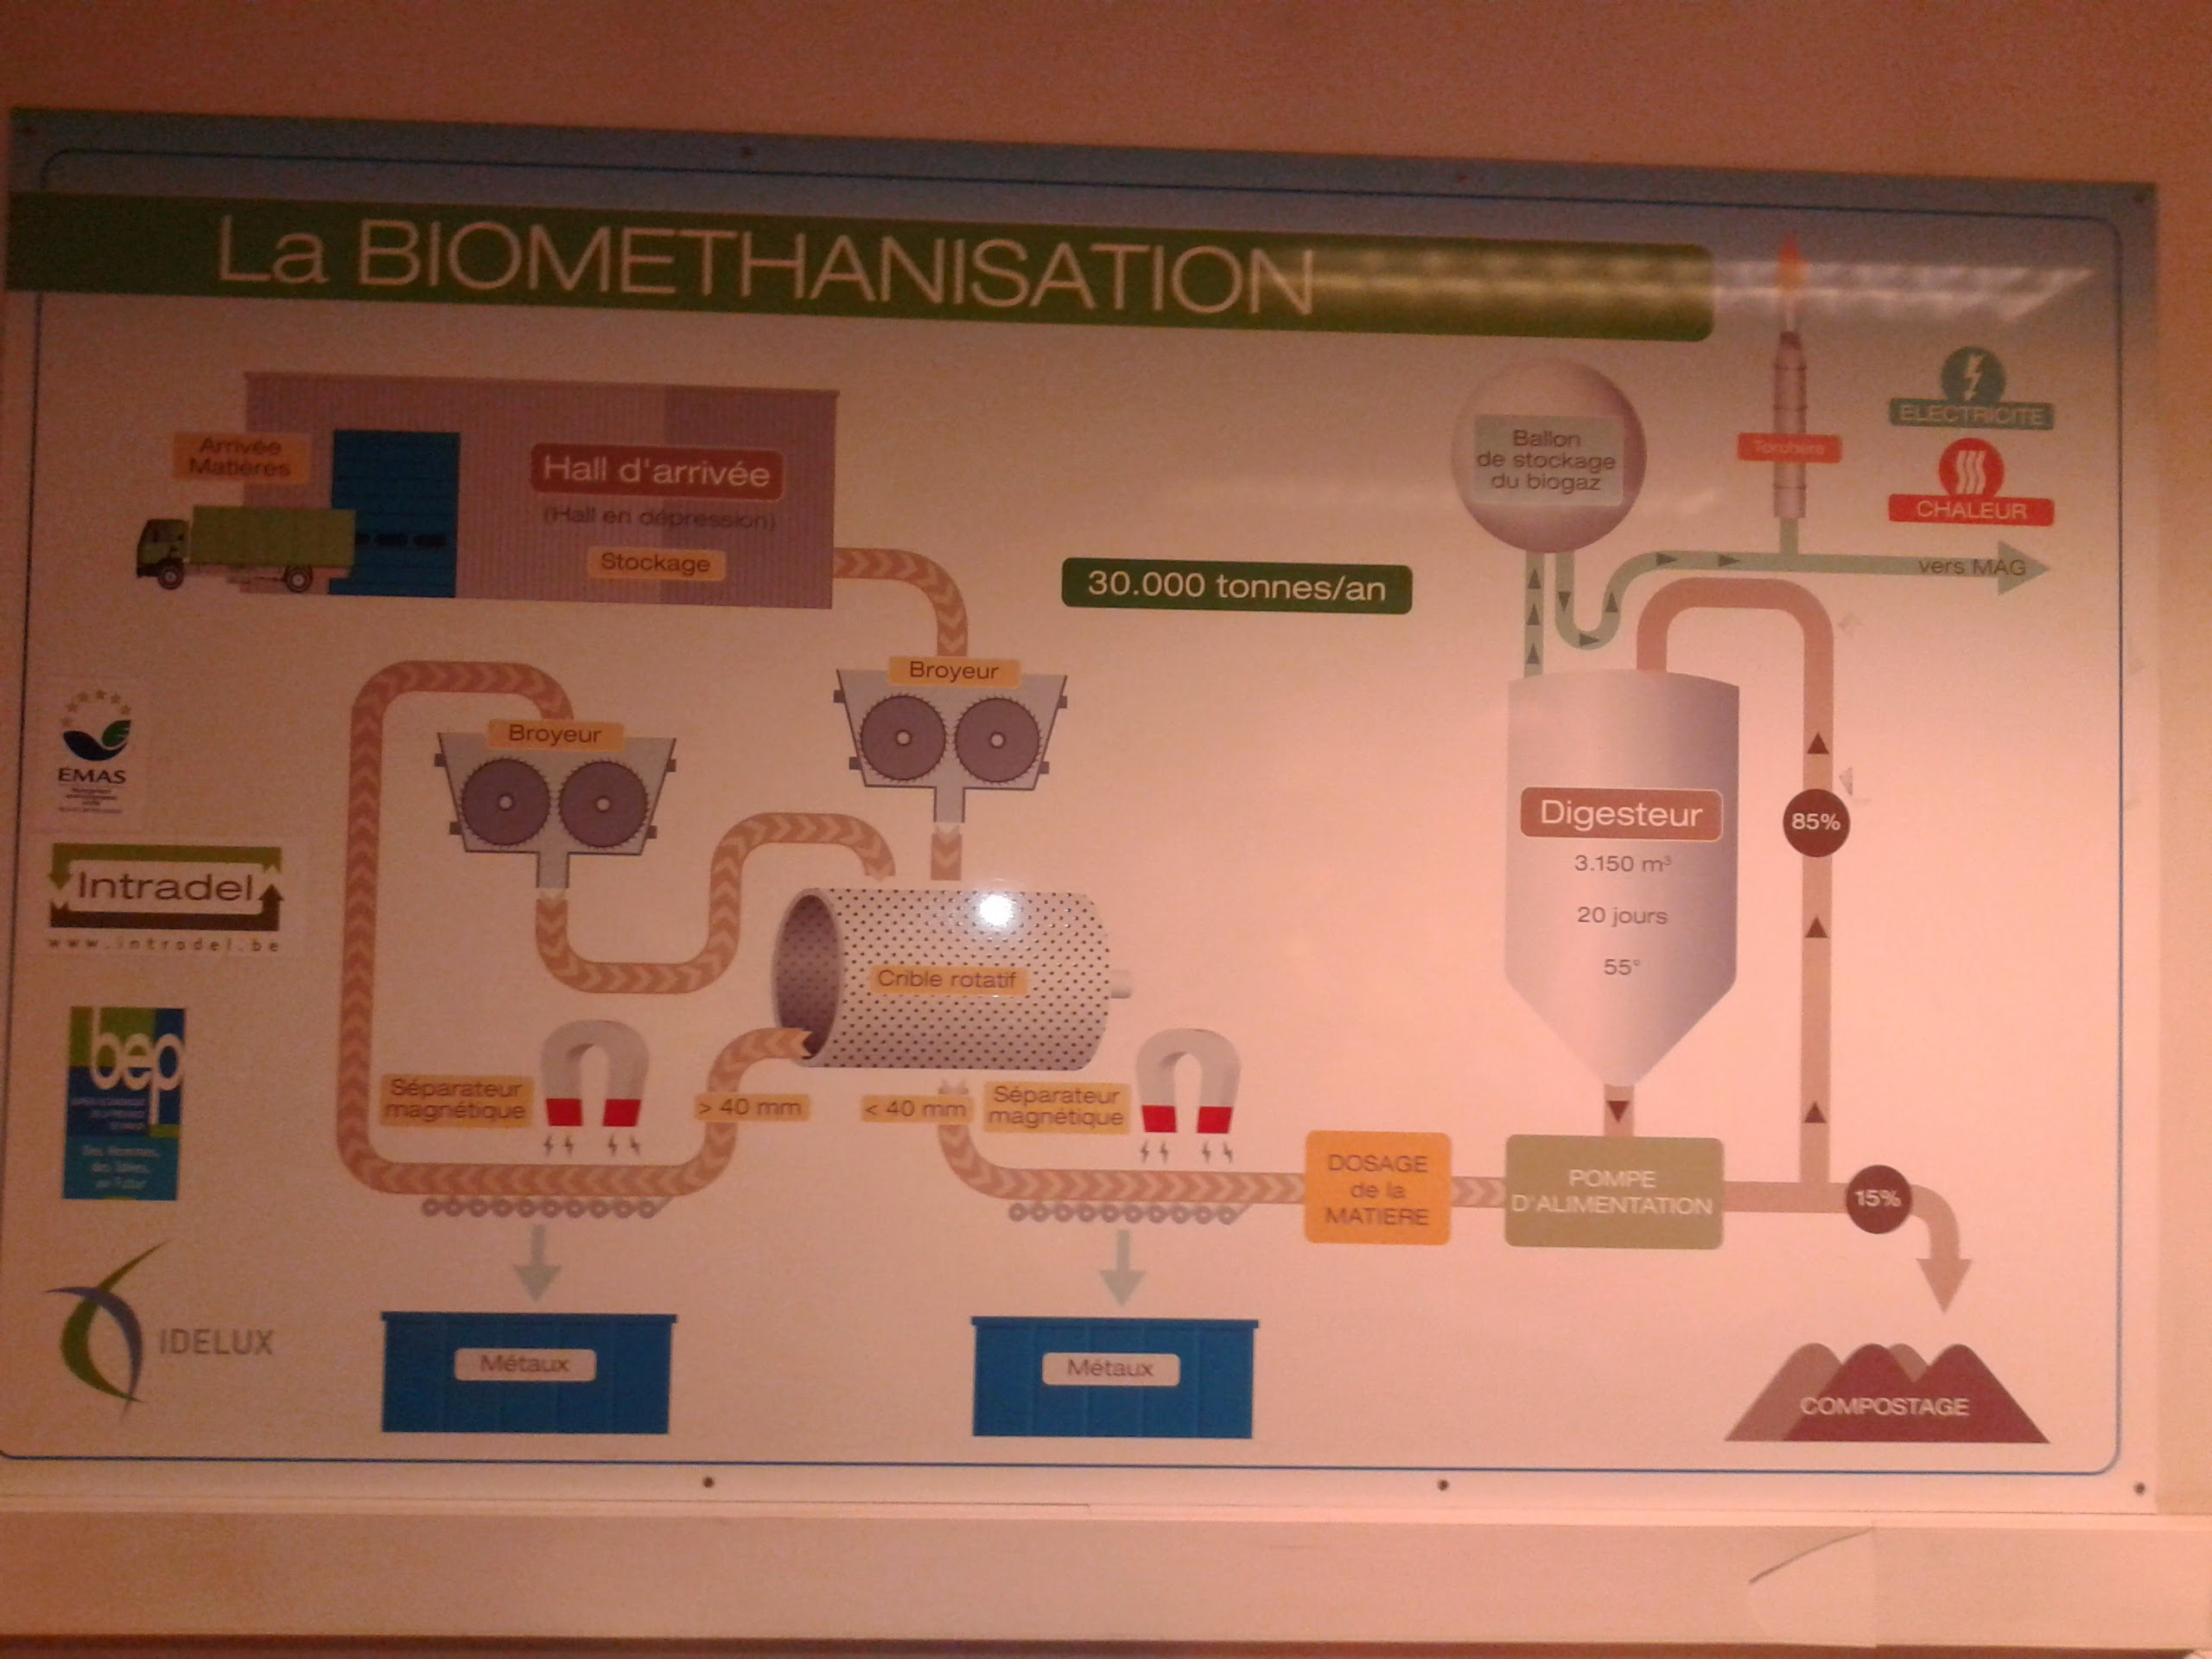
\includegraphics[scale=0.07]{IMG_20141105_105627.jpg}
  \caption{bio-méthanisation}
  \label{fig:biomethanisation}
\end{figure}
\subsection{Collecte des déchets}
Le centre de Tenneville récolte les déchets organiques de cuisine de plusieurs communes ainsi que tous les déchets ménagers de la commune du Luxembourg (\unit{240}{tonnes/an}). Elle collecte aussi les déchets verts et les PMC qui eux seront envoyés dans d'autres centres de tri.
A leur arrivée, les déchets de cuisine sont malheureusement pollués par, entre autre, des plastiques  et des métaux. Afin d'éliminer ces indésirables, les déchets passent dans un premier broyeur et les métaux sont récupérés grâce à un grand aimant (figure~\ref{fig:biomethanisation}). 
\subsection{Digesteur}
\begin{figure}
  \centering
  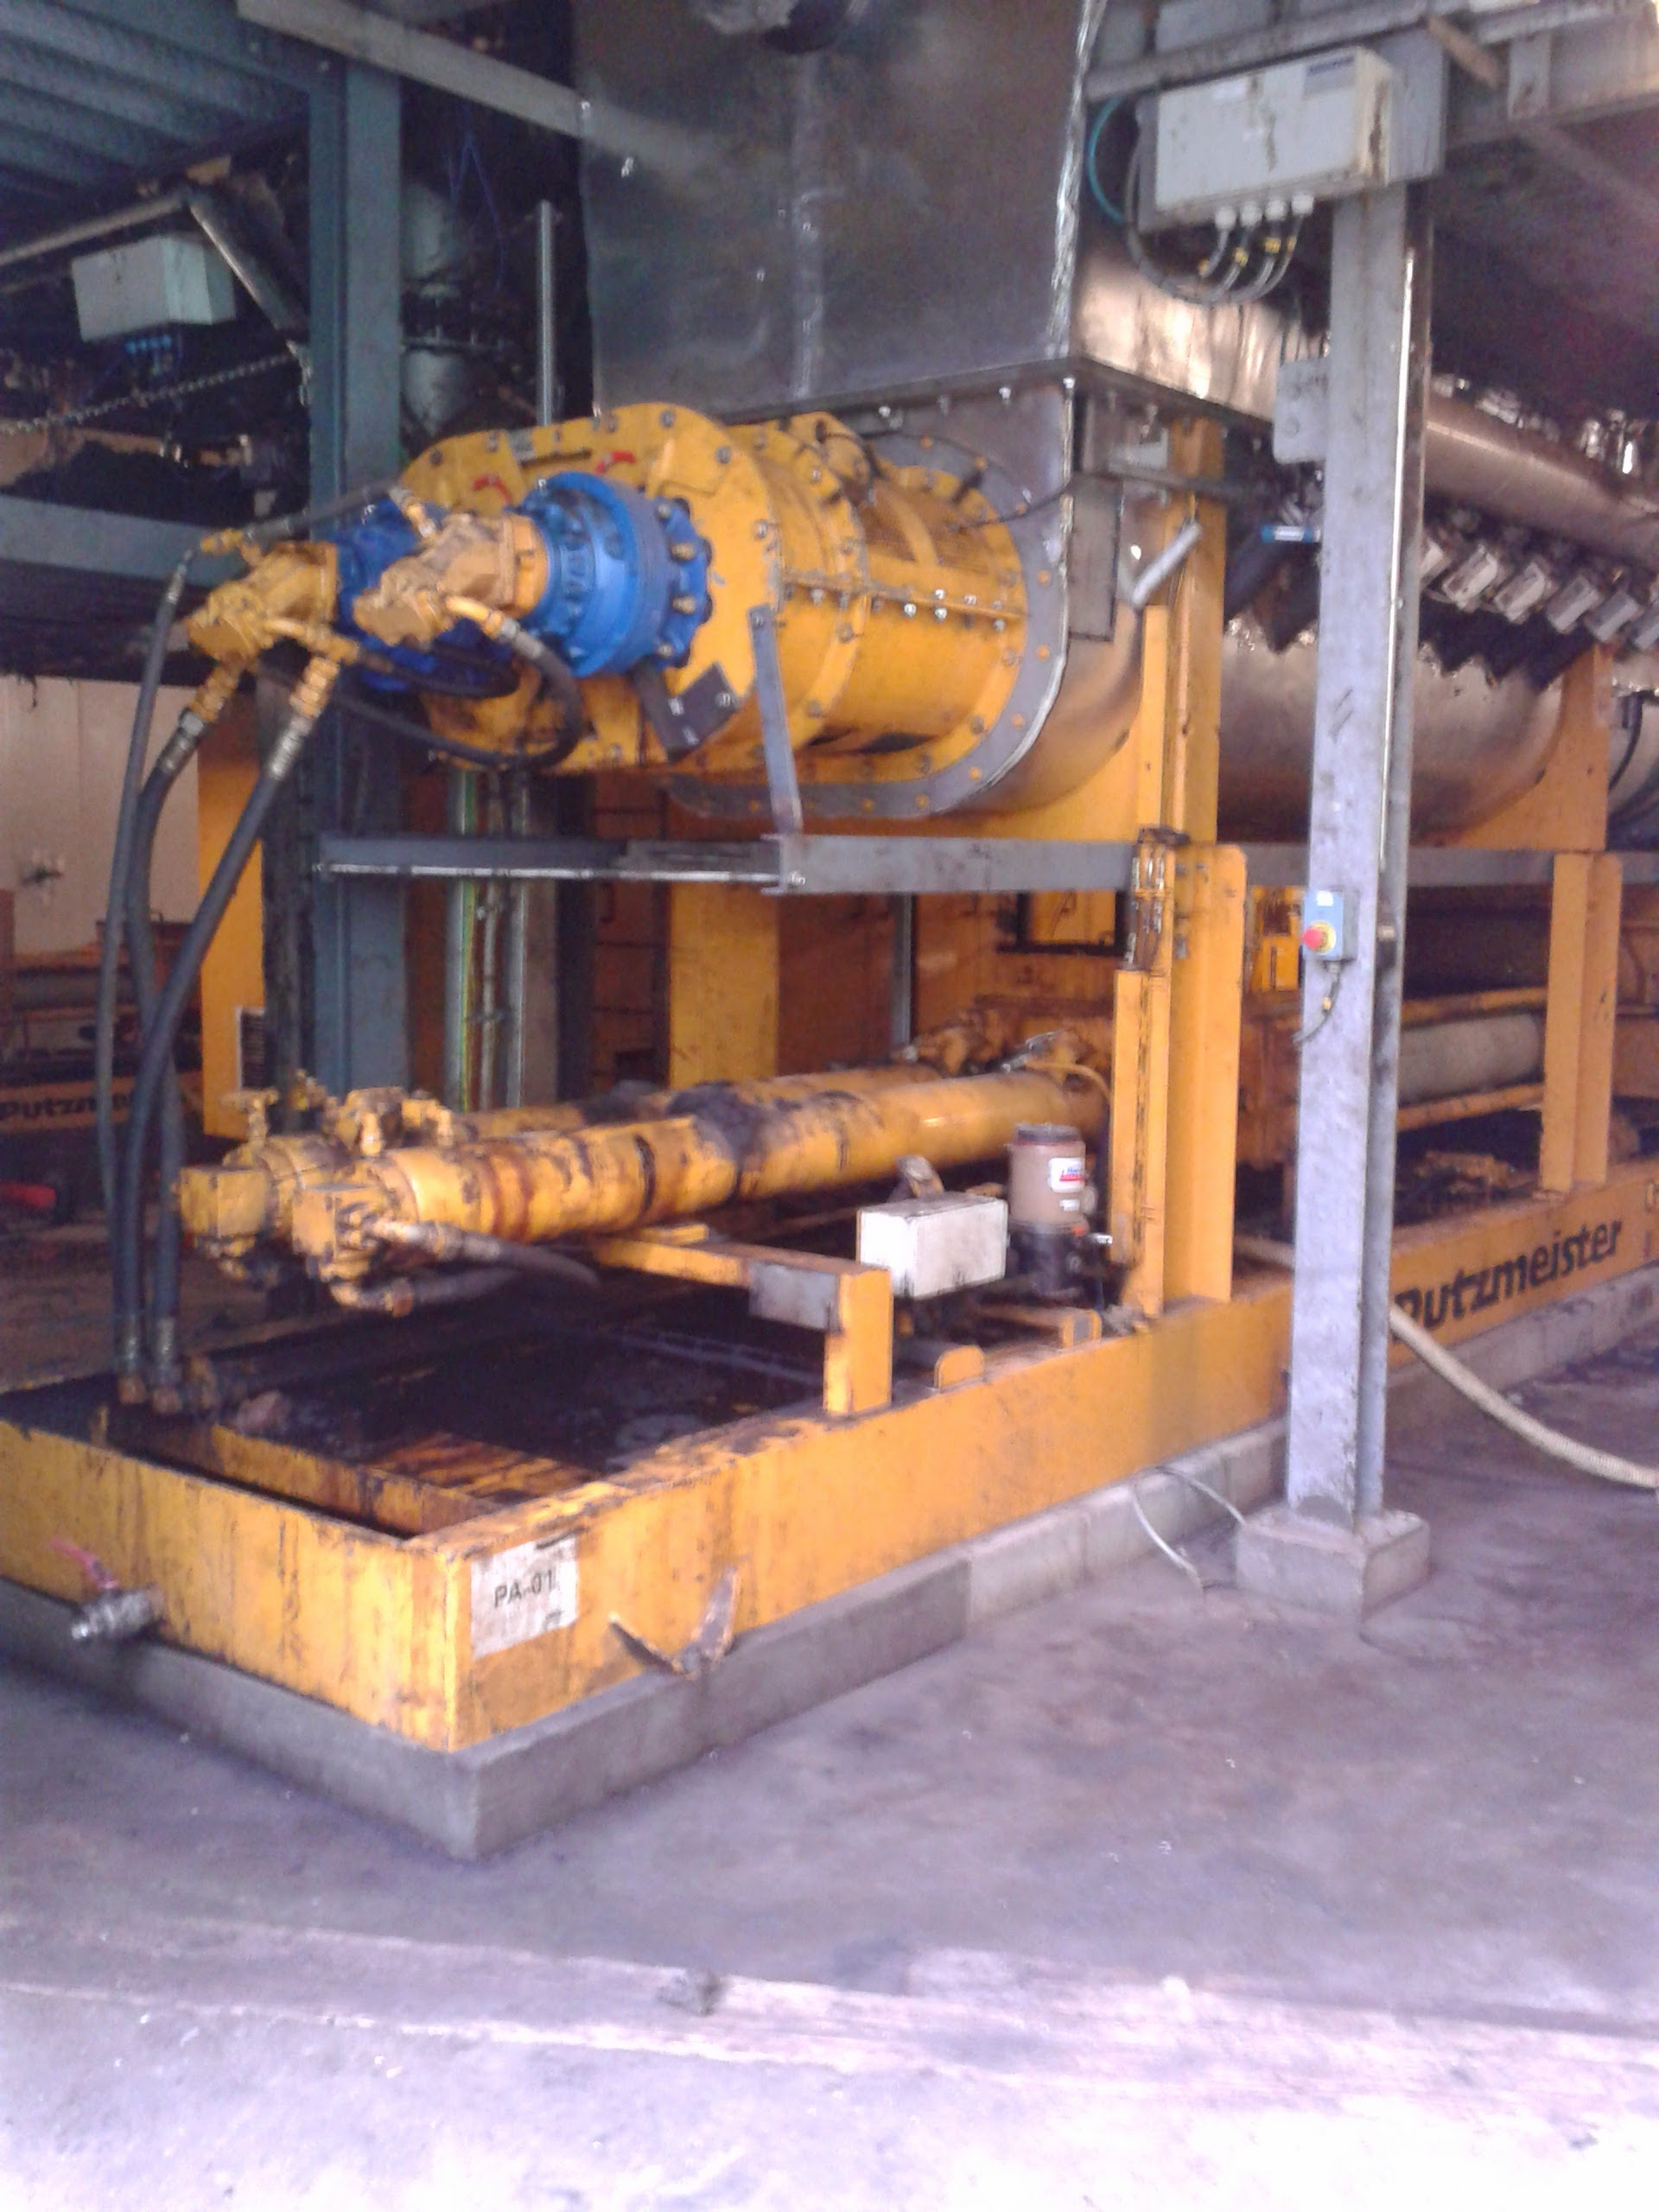
\includegraphics[scale=0.07]{IMG_20141105_112953.jpg}
  \caption{Digesteur}
  \label{fig:digesteur}
\end{figure}
Le digesteur est une cuve de \unit{3000}{m^3} qui fonctionne comme un grand estomac en 4 étapes: 
\begin{itemize}
\item Dégradation enzymatique
\item Acidogénèse
\item Acétogénèse
\item Méthanogénèse
\end{itemize}
A Tenneville, le digesteur monte à \unit{41}{\celsius}-\unit{43}{\celsius}  et son rendement est caractéristique à celui d'un procédé thermophile bien que la température habituelle d'un thermophile soit plutôt de \unit{55}{\celsius}. 

Le mélange injecté, via une pompe à piston, dans le digesteur est composé à \unit{85}{\%} de digesta et à \unit{15}{\%} de déchets frais. La matière y circule en moyenne 3 fois (20 jours) et ressort dans une consistance semblable à celle d'une bouse de vache (\unit{30}{\%} d'humidité).

C'est au sommet du digesteur qu'est récolté le biogaz (\unit{50}{\%} de méthane, \unit{30}{\%} de \ce{CO2}, de l'eau, de l'hydrogène sulfuré (\ce{H2S}) et de l'oxygène). Le digesteur de Tenneville produit environs \unit{1000}{m^3/h}.
Le méthane est alors transformé en électricité grâce à un moteur et produit assez pour que l'installation ne consomme que \unit{2.4}{\%} d'électricité du secteur et permet même de vendre \unit{7000}{MW/an}. De la chaleur est aussi produite, celle-ci est utilisée par 5 choses:
\begin{enumerate}
\item Chauffer les bâtiments de l'installation.
\item Chauffer des bâtiments communaux.
\item Faire sécher les boues (figure~\ref{fig:Secheur}) de la station d'épuration (\unit{700}{kW/an}).
\item Chauffer les eaux récoltées dans la décharge.
\item Par une société qui recycle le plastique afin de faire des plastiques agricoles.
\end{enumerate}
\begin{figure}
  \centering
  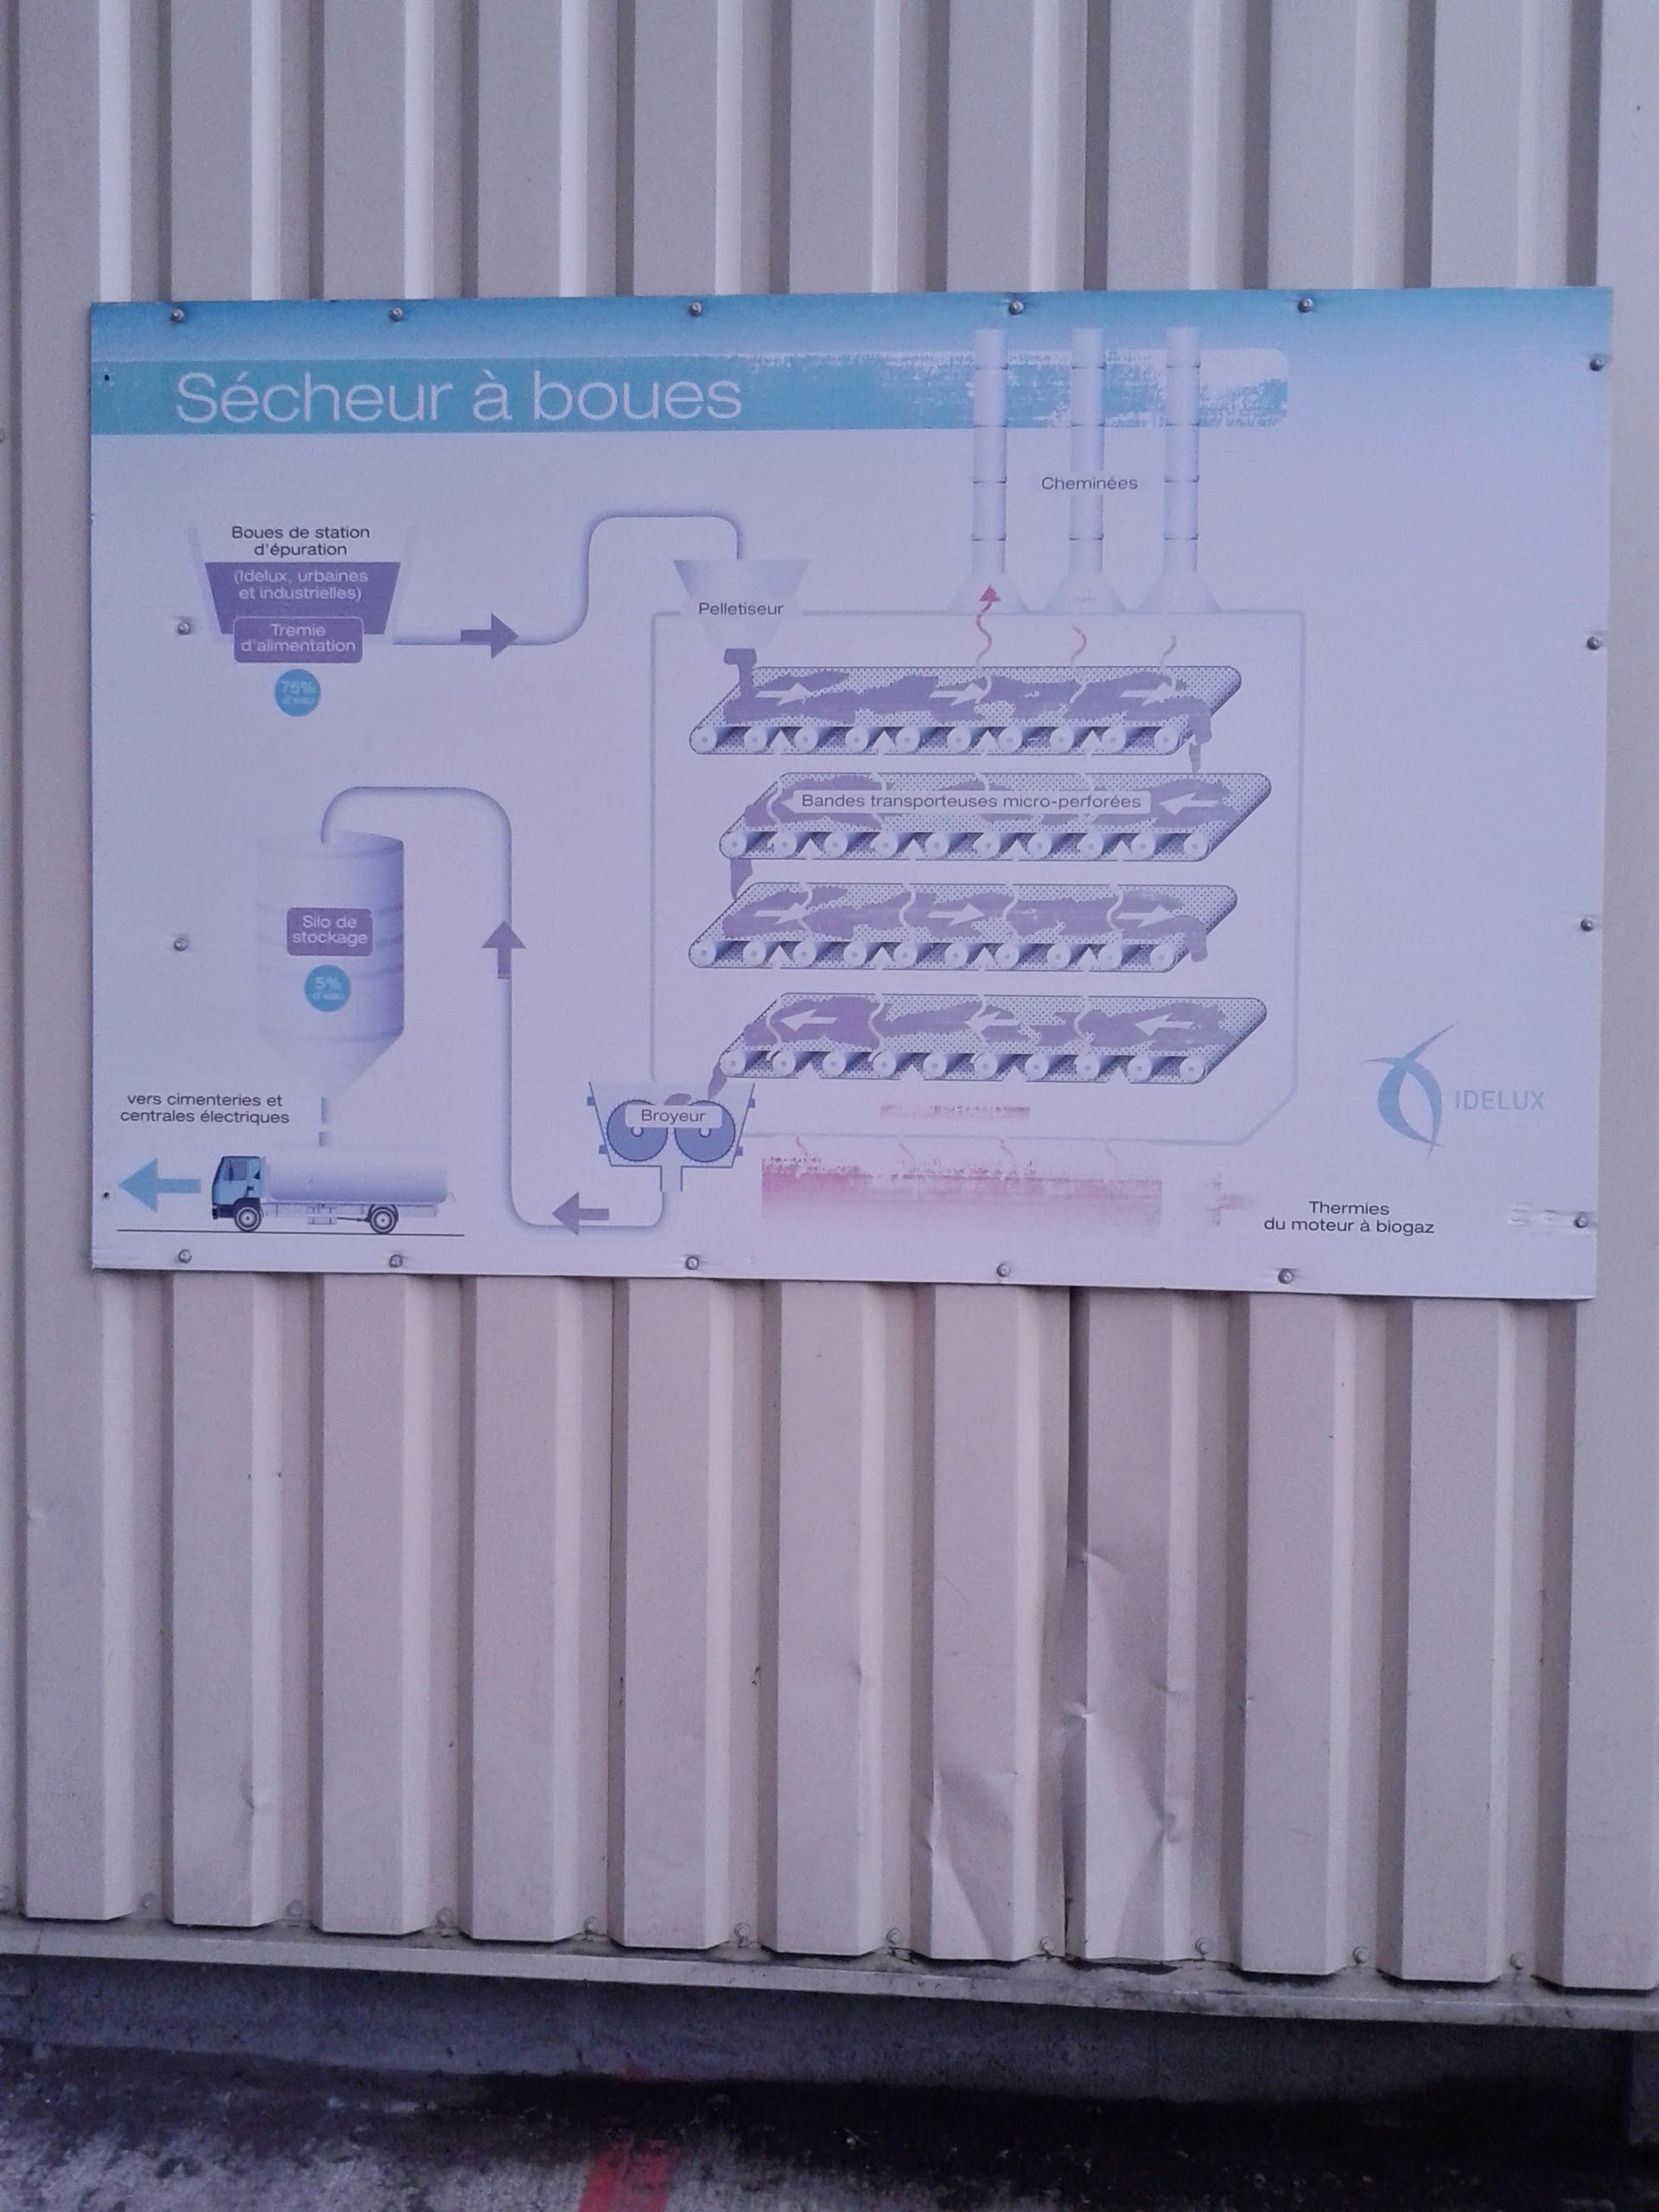
\includegraphics[scale=0.07]{IMG_20141105_113638.jpg}
  \caption{Sécheur à boue}
  \label{fig:Secheur}
\end{figure}
\subsection{Le compostage}
Le compostage se fait par bio-séchage de 2-3 semaines du digesta ainsi que de déchets verts. Pour ce faire, le mélange est placé sur des dalles où de l'air va circuler afin de garder un taux d'oxygène assez élevé tout en gardant une chaleur avoisinant les \unit{60}{\celsius}.
\begin{figure}
  \centering
  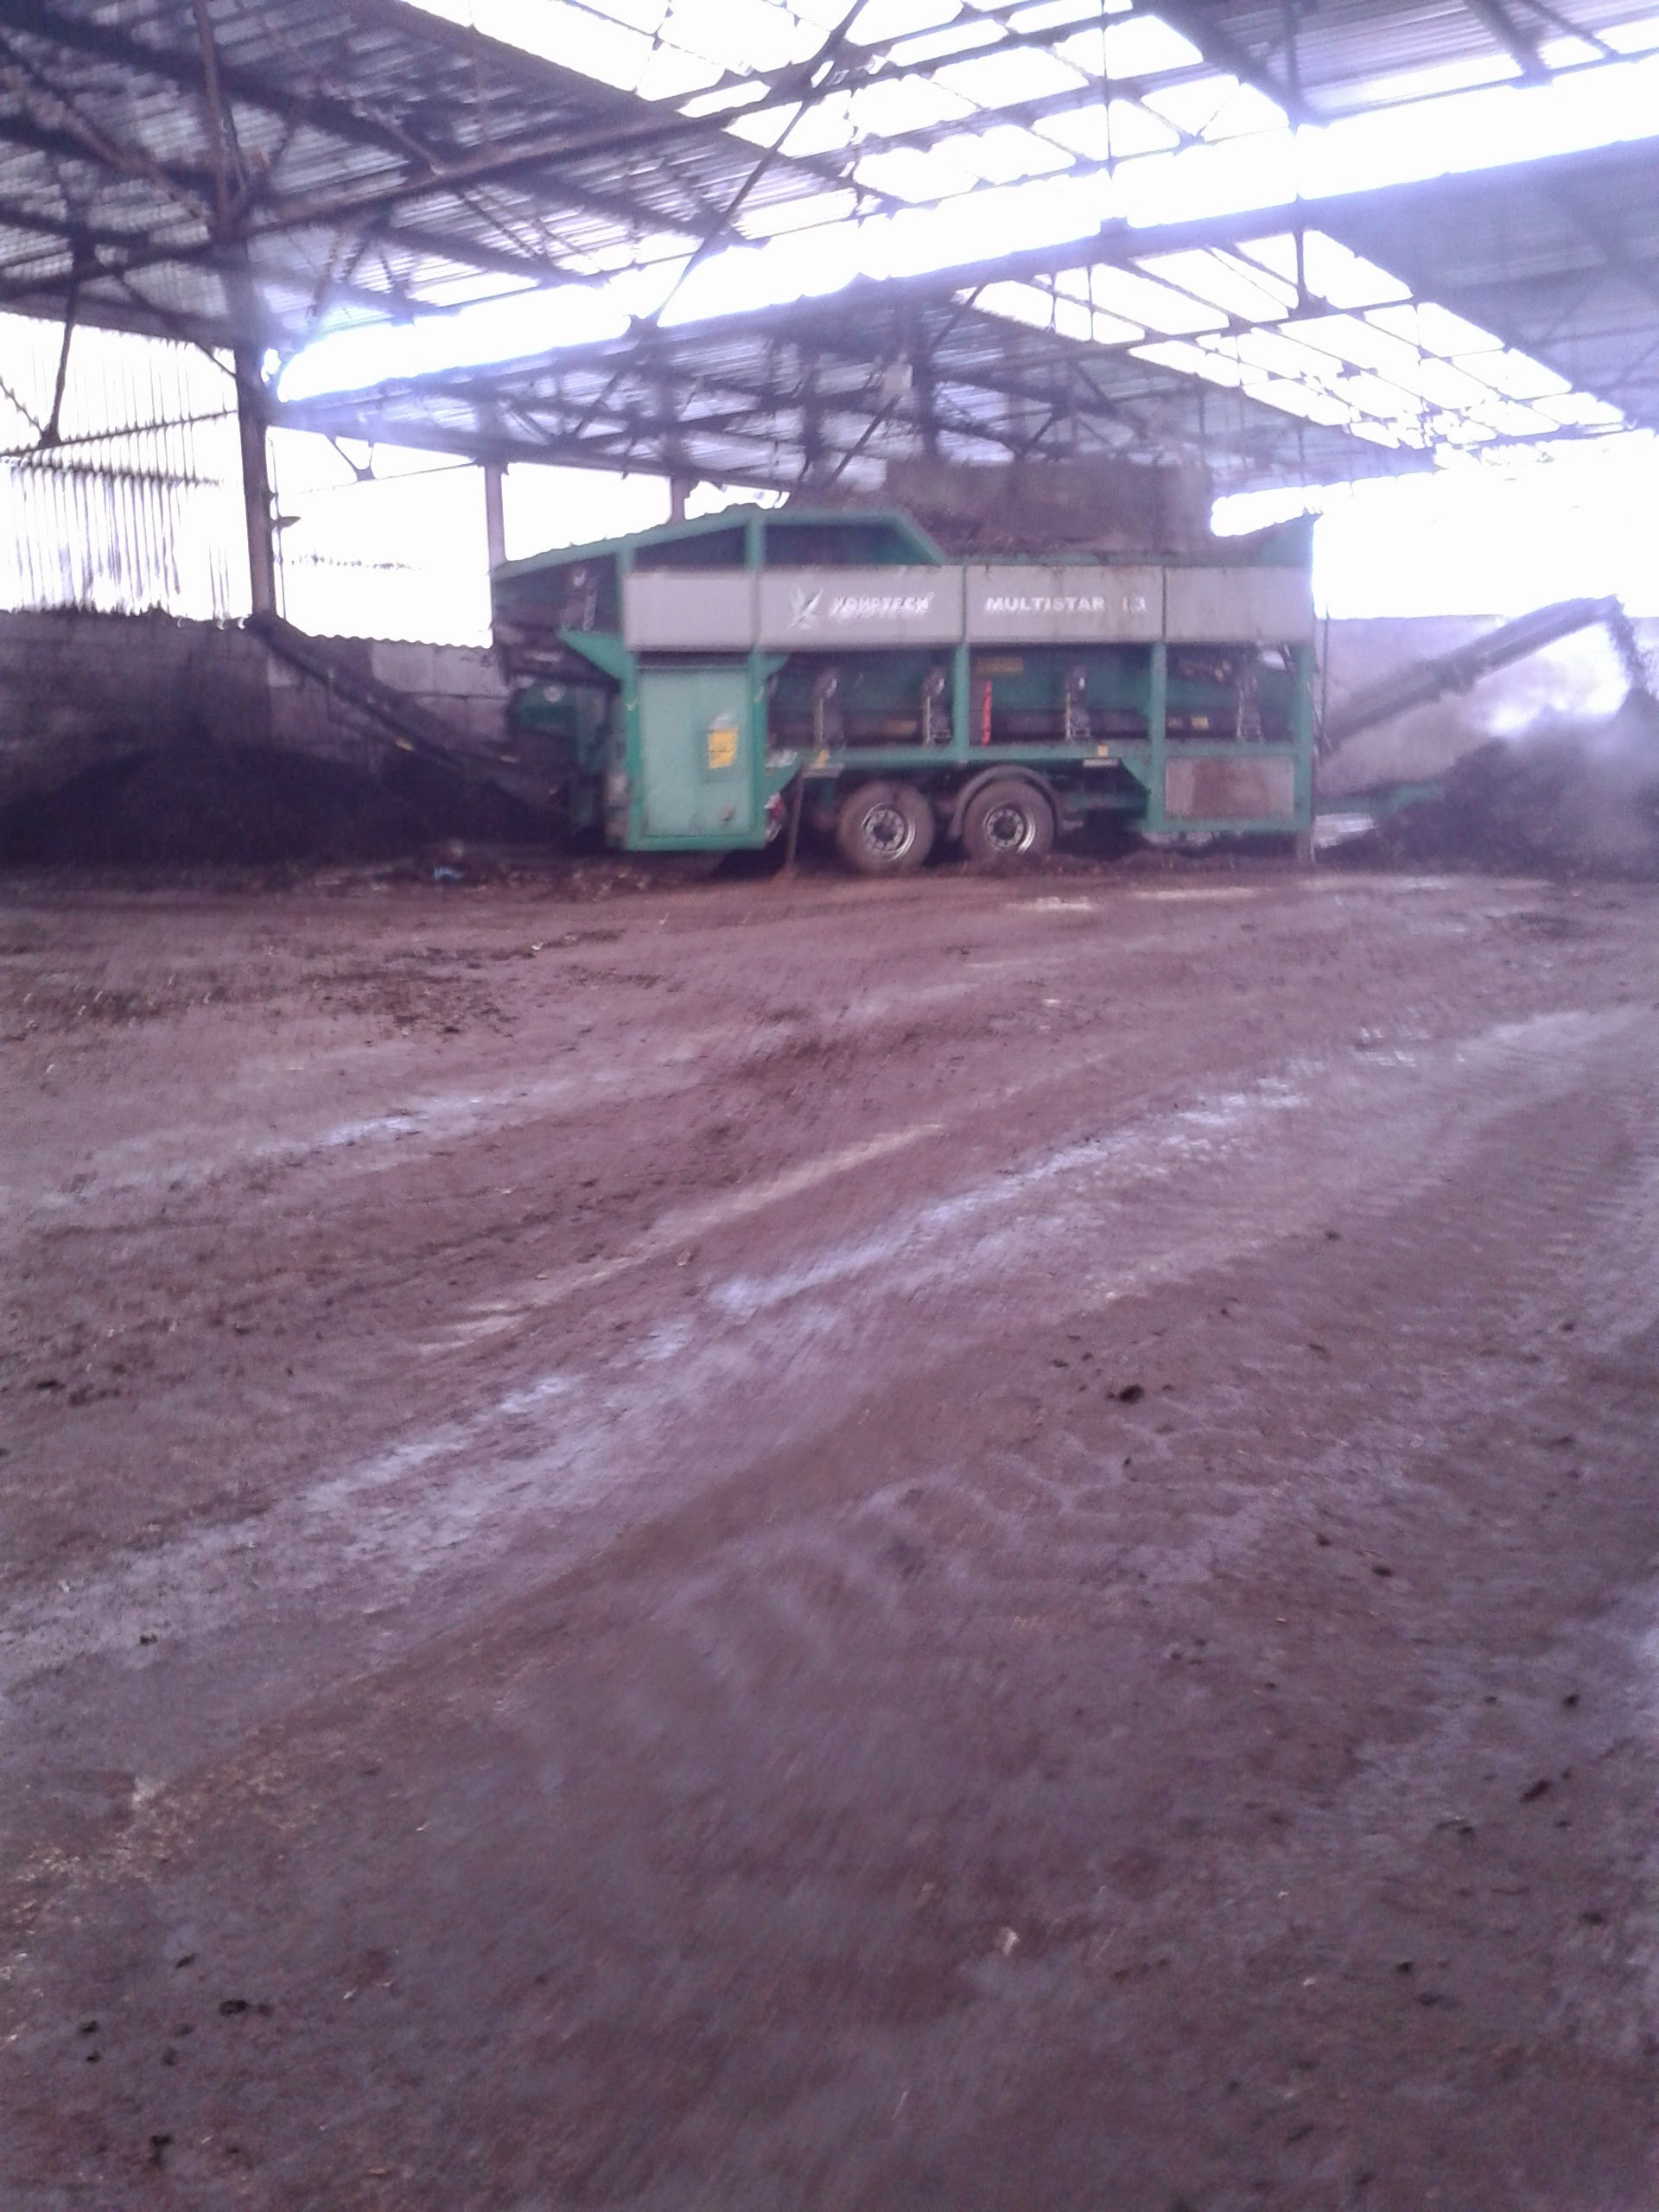
\includegraphics[scale=0.07]{IMG_20141105_102726.jpg}
  \caption{Tamiseur}
  \label{fig:tamiseur}
\end{figure}
Le mélange passe alors dans une machine à tamis (figure~\ref{fig:tamiseur}) qui le sépare en 3 tas:
\begin{enumerate}
\item Granulométrie $< \unit{12}{mm}$ (figure~\ref{fig:Granu12}).
\item Granulométrie $< \unit{20}{mm}$.
\item Granulométrie $> \unit{20}{mm}$ (figure~\ref{fig:granumore20}).
\end{enumerate}
\begin{figure}
  \centering
  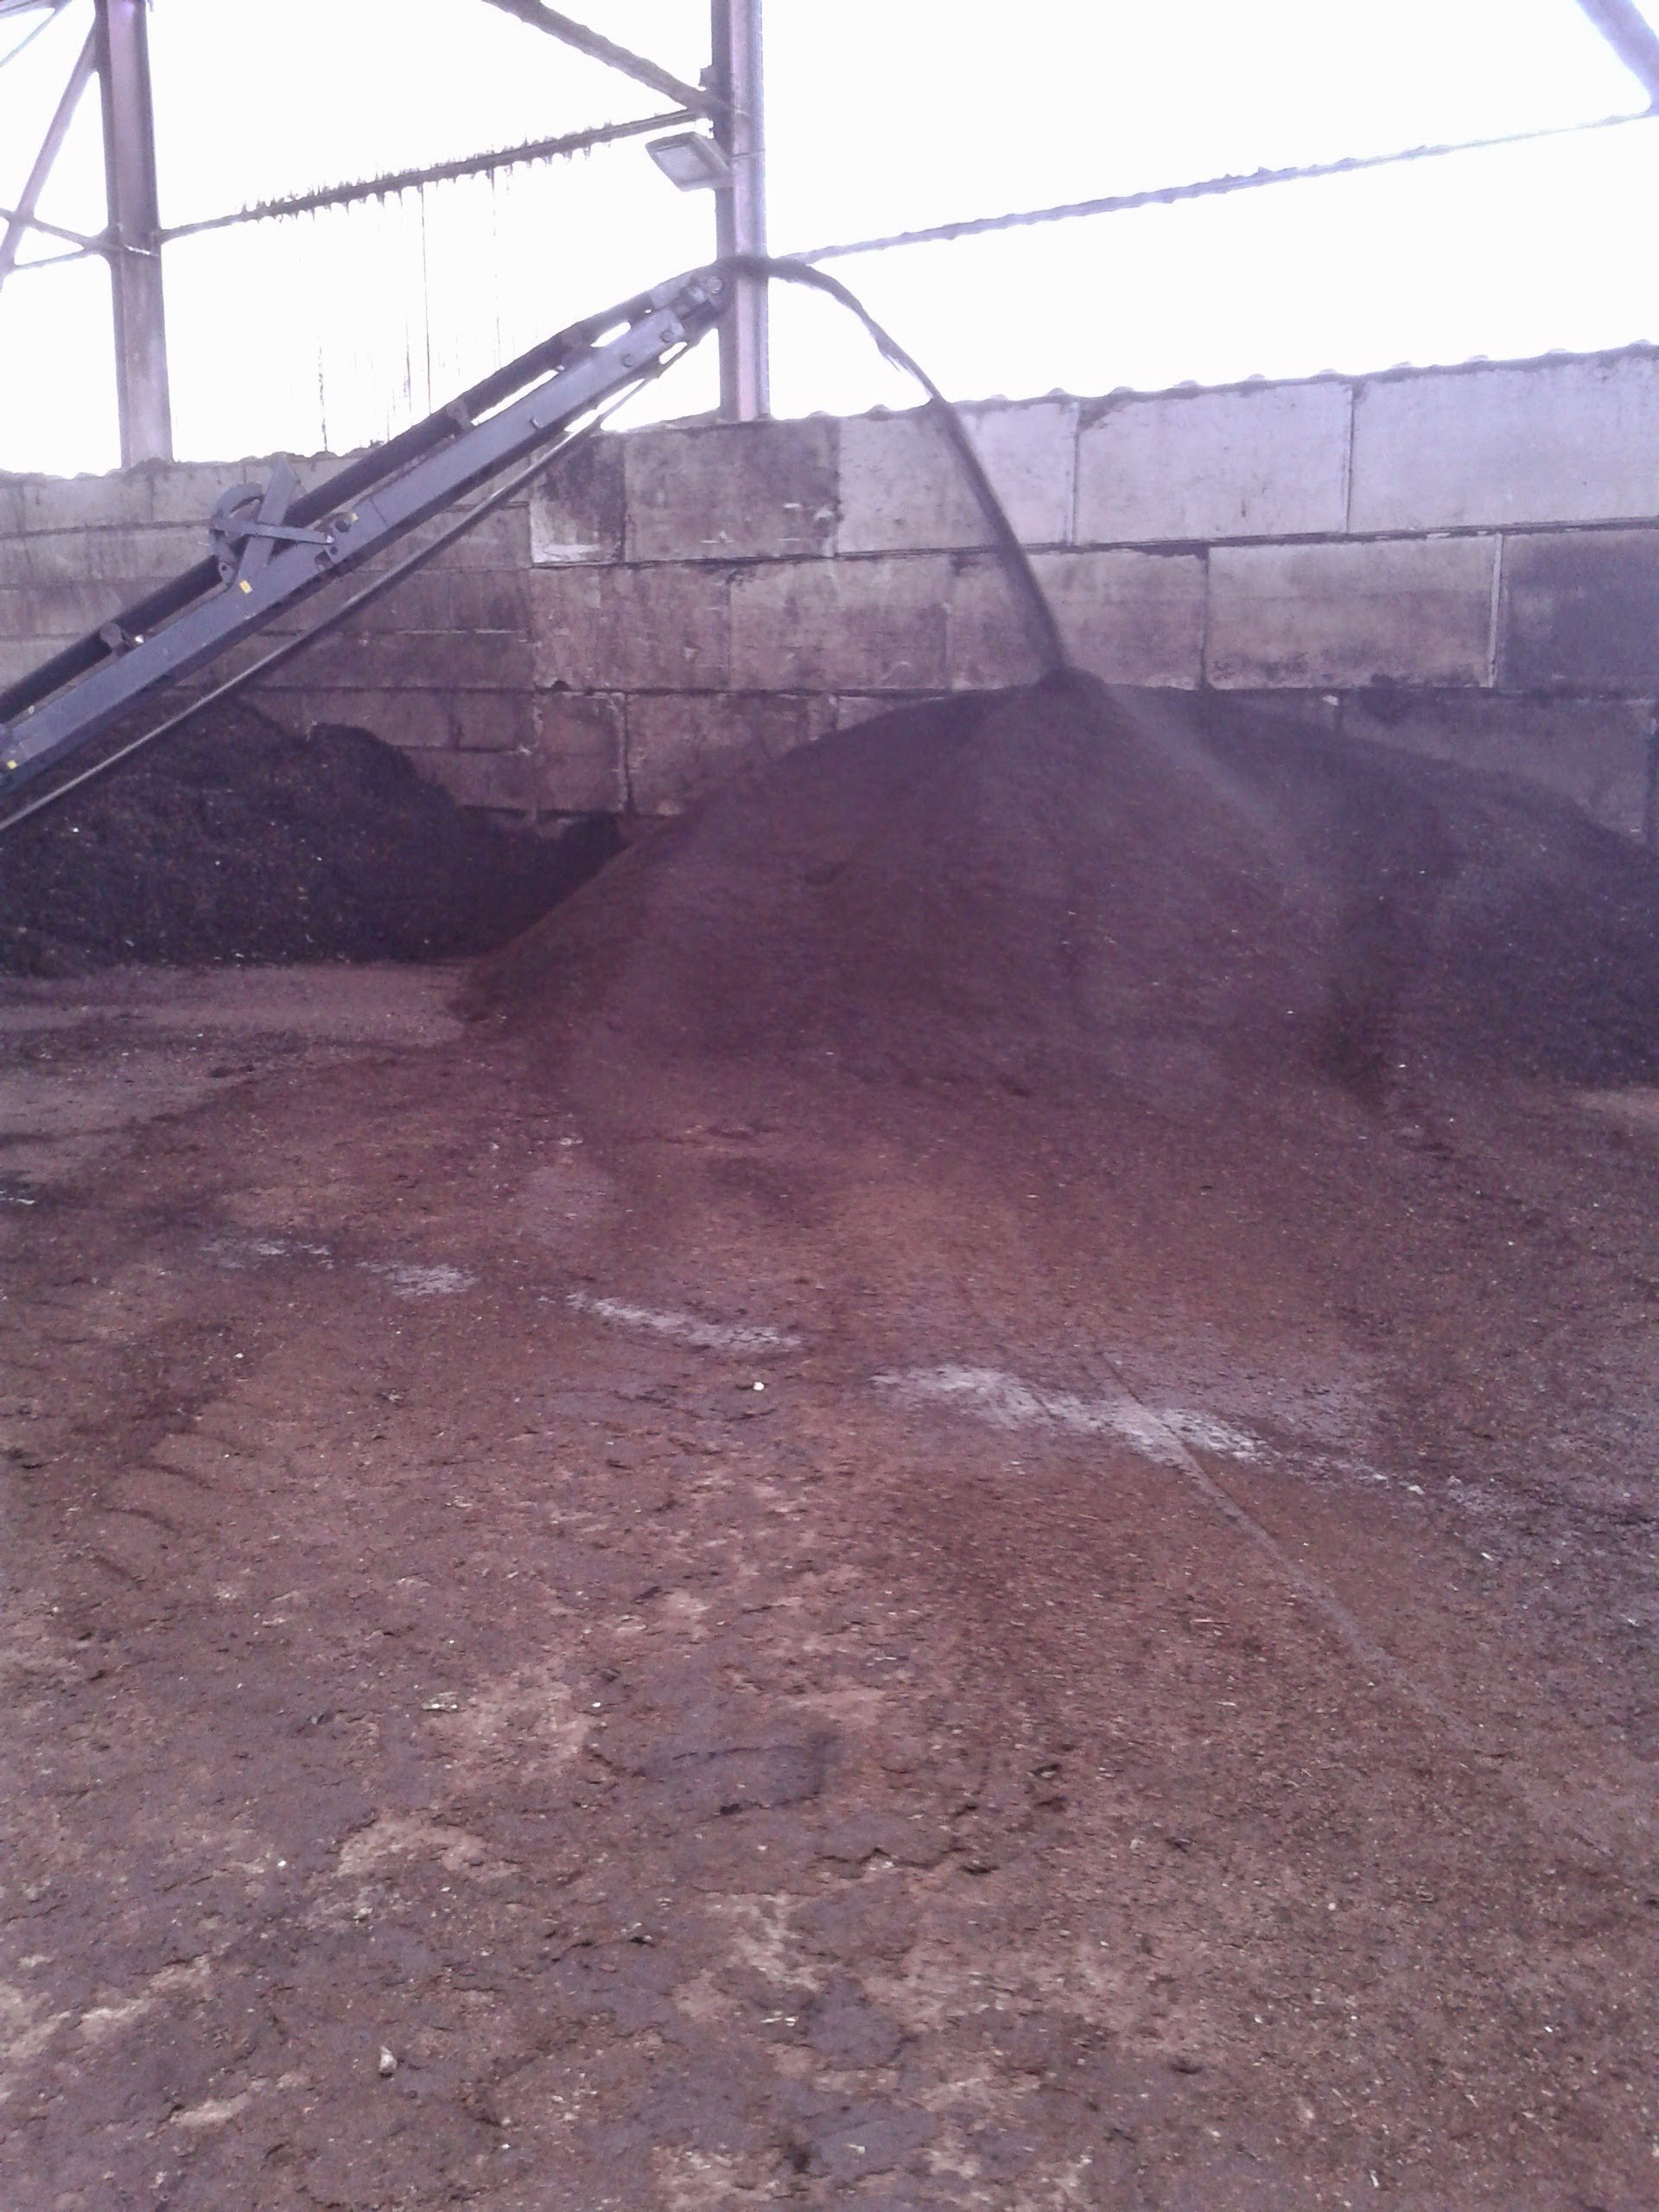
\includegraphics[scale=0.07]{IMG_20141105_103027.jpg}
  \caption{Granulométrie $< \unit{12}{mm}$}
  \label{fig:Granu12}
\end{figure}
\begin{figure}
  \centering
  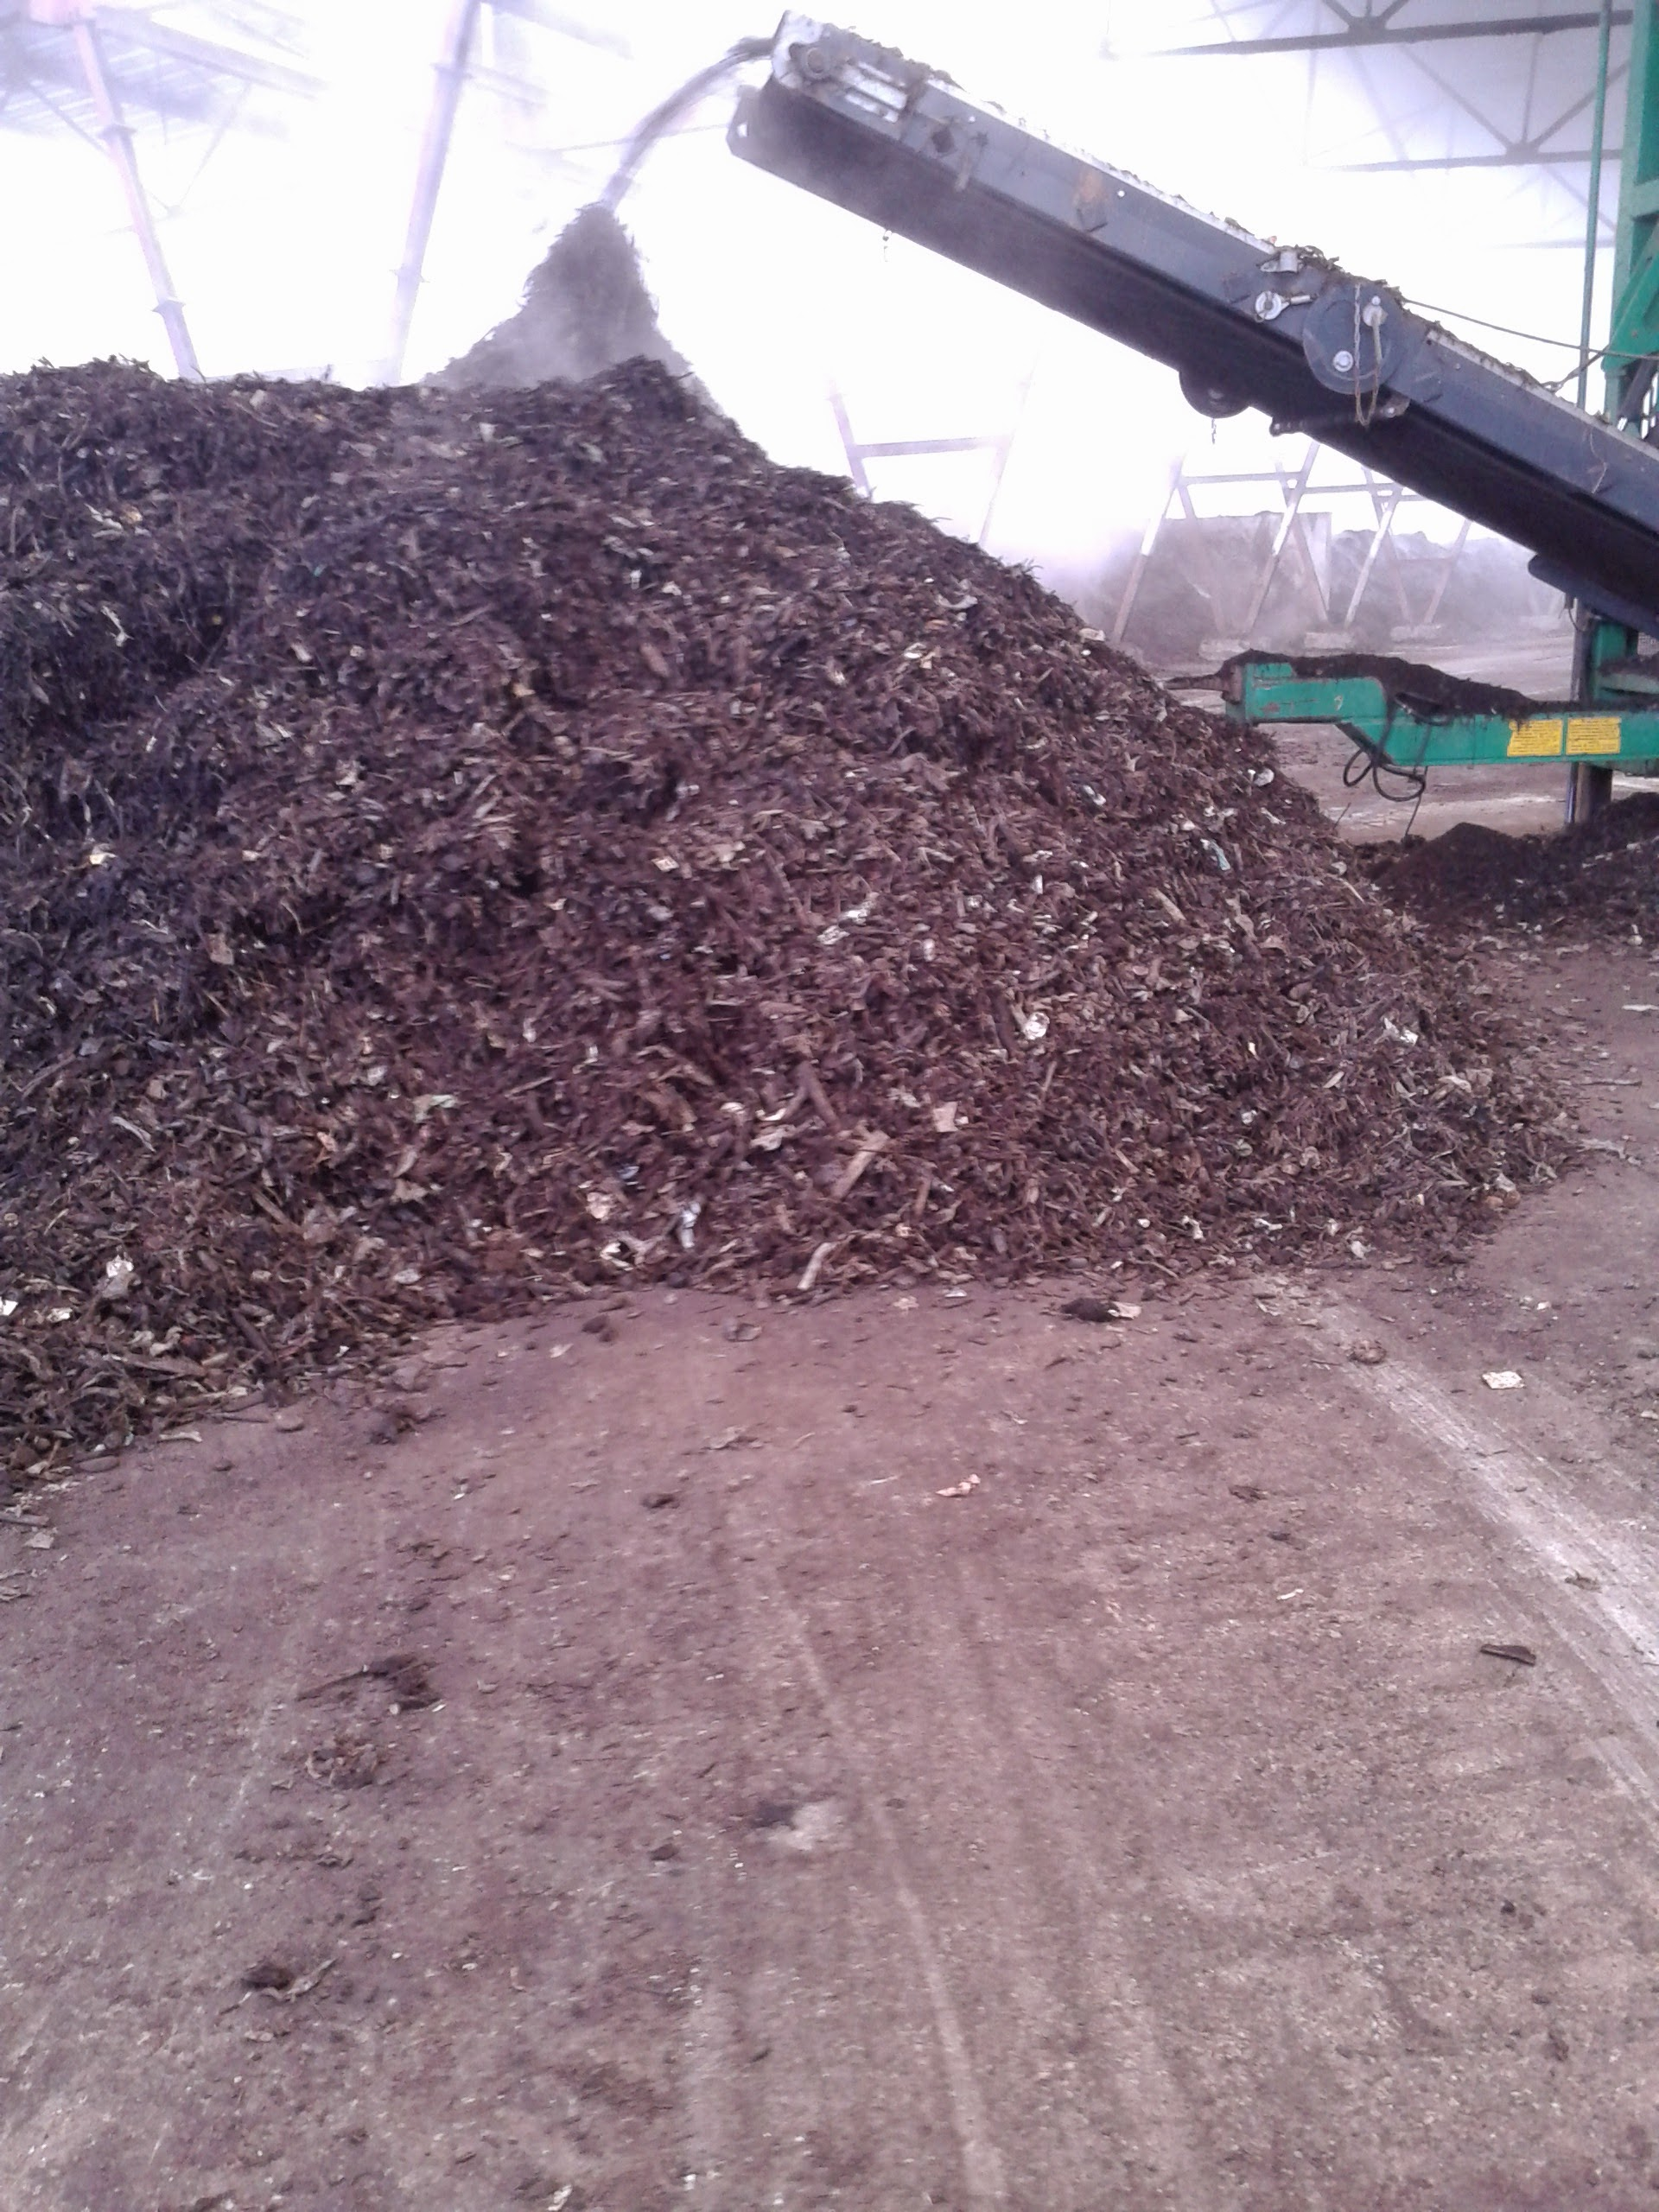
\includegraphics[scale=0.07]{IMG_20141105_103019.jpg}
  \caption{Granulométrie $> \unit{20}{mm}$}
  \label{fig:granumore20}
\end{figure}
La coupure avec une granulométrie supérieure à \unit{20}{mm} pourra être réinjectée dans le cycle tandis que celle avec une granulométrie inférieure à \unit{12}{mm} subira un traitement de maturation de 6 à 8 semaines afin d'être revendue 5 euro la tonne comme terreau.

En hiver, afin d'avoir une température suffisante, de la chaux vive sera ajoutée (le terreau pourra alors être vendu 8 euro la tonne).
\section{Conclusion}
Pour notre projet, il serait intéressant de se coupler avec une telle installation. En effet, celle-ci produit du méthane et de la chaleur tout en ayant un impact positif sur l'environnement.

Acheter le méthane qui transiterait via gazoduc, serait peut-être aussi à explorer bien que cette possibilité ne soit pas envisageable à Tenneville.

\end{document}


\appendix
\chapter{Bilan de masse: annexes}

\section{Système linéaire du bilan de masse}\label{appendix:matrix}

Pour éventuellement aider à comprendre le fonctionnement du bilan de masse, nous fournissons ici le système, sous forme matriciel, qui est à résoudre pour obtenir l'espace vectoriel $V$.

Dans l'ordre, les lignes de la matrice correspondent aux composés suivants : \ce{CH4}, \ce{H2O}, \ce{O2}, \ce{N2}, \ce{Ar}, \ce{CO},  \ce{CO2}, \ce{H2} et \ce{NH3}.
\[
\left(
\begin{array}{*{12}c}
  1 & 0 & 0 & 0 & 0 & 0 & 0 & -1 & 0 & -2 & 0 & 0 \\
  0 & 1 & 0 & -1 & 0 & 0 & 0 & -1 & -1 & 0 & -1 & 0 \\
  0 & 0 & 0 & 0 & 0 & 0 & 0 & 3 & 1 & 4 & 1 & -3 \\
  0 & 0 & 0 & 0 & 0 & 0 & 0 & 1 & -1 & 2 & -1 & 0 \\
  0 & 0 & 0 & 0 & -1 & 0 & 0 & 0 & 1 & 0 & 1 & 0 \\
  0 & 0 & .21 & 0 & 0 & 0 & 0 & 0 & 0 & -1 & 0 & 0 \\
  0 & 0 & .78 & 0 & 0 & 0 & 0 & 0 & 0 & 0 & 0 & -1 \\
  0 & 0 & .01 & 0 & 0 & -1 & 0 & 0 & 0 & 0 & 0 & 0 \\
  0 & 0 & 0 & 0 & 0 & 0 & -1 & 0 & 0 & 0 & 0 & 2
\end{array}
\right)
\left(
\begin{array}{*{1}c}
  n_{i,\ce{CH4}} \\ n_{i,\ce{H2O}} \\ n_{i,\text{air}} \\ n_{f,\ce{H2O}} \\ n_{f,\ce{CO2}} \\ n_{f,\ce{Ar}} \\ n_{f,\ce{NH3}} \\ R_1 \\ R_2 \\ R_3 \\ R_4 \\ R_5
\end{array}
\right)
= 0
\]


\section{Calcul des constantes d'équilibre}\label{appendix:const_eq}

Nous avons calculé les constantes d'équilibre des réactions 1 et 2 avec Matlab, à l'aide de l'expression suivante :
\[
    K = \mathrm{exp}\!\left( -\frac{\Delta G^0_m(T)}{RT} \right)
      = \mathrm{exp}\!\left( \frac{\Delta S^0_m(T)}{R} - \frac{\Delta H^0_m(T)}{RT} \right)
    \text.
\]
Dans cette expression, le symbole $\Delta$ correspond à la différence entre les produits et les réactifs. Par exemple, $\Delta S^0_m(T)$ est la somme de l'entropie molaire des produits moins l'entropie molaire des réactifs.

Il est donc nécessaire d'obtenir $\Delta S^0_m(T)$ et $\Delta H^0_m(T)$. Ceux-ci sont calculés à l'aide des formules :
\[
    \Delta S^0_m(T) = \Delta S^0_m(T_0) + \int_{T_0}^T\! \Delta C_{p,m} \frac{\diff{T}}{T}
    \qquad\text{et}\qquad
    \Delta H^0_m(T) = \Delta H^0_m(T_0) + \int_{T_0}^T\! \Delta C_{p,m} \diff{T}
    \text.
\]
Enfin, la différence de capacités calorifiques molaires $\Delta C_{p,m}$ qui apparait ici est obtenue, sous forme de polynomes de $T$, dans des tables thermodynamiques. Il en va de même pour l'enthalpie et l'entropie à la température de référence $T_0$.

Nous avons donc tous les outils nécessaires pour calculer la valeur de $K$ dans les deux réactions du réformeur primaire. Il suffit simplement d'implémenter les formules dans Matlab pour obtenir les constantes d'équilibres utilisées dans le calcul du bilan de masse.


\section{Usage du programme Matlab}

Le programme Matlab se trouve dans le sous-dossier \texttt{/manager/}. Il s'agit de la fonction \texttt{manager(m\_NH3, T\_reformer)}, qui elle-même utilise d'autres fonctions, également présentes dans le répertoire.

Une explication concise du fonctionnement de la fonction peut être trouvée en utilisant \texttt{help manager} dans la ligne de commande Matlab.


\section{Flowsheet}\label{appendix:flowsheet}

\tikzstyle{decision} = [diamond, draw, fill=blue!20,
    text width=4.5em, text badly centered, node distance=3cm, inner sep=0pt]
\tikzstyle{block} = [rectangle, draw, fill=blue!20,
    text width=14em, text centered, rounded corners, minimum height=4em, minimum width=15em, node distance=3cm]
\tikzstyle{block2} = [rectangle, draw, fill=red!20,
    text width=14em, text centered, rounded corners, minimum height=4em, minimum width=15em, node distance=3cm]
\tikzstyle{line} = [draw, -latex']
\tikzstyle{cloud} = [draw, ellipse,fill=red!20, node distance=3cm,
    minimum height=2em]

\begin{figure}
	\begin{tikzpicture}[node distance = 3cm, auto]
	    % Place nodes
	    \node [block] (RefPrim) {\textbf{Réformage primaire}(Réformage à vapeur de \ce{CH_4}) $$\ce{CH_4 + H_2O \Leftrightarrow CO + 3H_2}$$ \textit{Equilibre à T (sortie)} };
	    \node [block2, left of=RefPrim, node distance=7cm] (Four) {\textbf{Four} \\ Combustion de \ce{CH_4} \\ \textit{Irreversible et complète}};
	    \node [block, below of=RefPrim, node distance=3.5cm] (RefSec) {\textbf{Réformage secondaire} $$\ce{2CH_2 + O_2 \Rightarrow}$$ \textit{Considérée comme irréversible et complète à la fin.}};
	    \node [block, below of=RefSec, node distance=3.5cm] (Reacteur) {\textbf{Réacteurs Water-Gas-Shift} $$\ce{CO + H_2O \Rightarrow CO_2 + H_2}$$ \textit{Considérée comme complète à la fin.} };
	    \node [block, below of=Reacteur, node distance=3.5cm] (AbsComp) {\textbf{Absorption de \ce{CO_2} et compression} (séparation d'\ce{H_2 O}) \\ \textit{Considérées complètes.}};
	    \node [block, below of=AbsComp, node distance=3.5cm] (Synth) {\textbf{Synthèse d'\ce{NH_3} et séparation} $$\ce{N_2 + 3H_2\Leftrightarrow 2NH_3}$$ \textit{Considérées complètes.}};
	    \node [right of =AbsComp, node distance=4cm] (nothing1){};
	    \node [below of =Synth] (nothing2){};
	    % Draw edges
	    \path [line] (RefPrim) -- (RefSec);
	    \path [line] (Four) -- (RefPrim);
	    \path [line] (RefSec) -- (Reacteur);
	    \path [line] (Reacteur) -- node {\ce{CO_2 + H_2}} (AbsComp);
	    \path [line] (AbsComp) -- (Synth);
	    \path [line] (AbsComp) -- node {\ce{CO_2(l)}}(nothing1);
	    \path [line] (Synth) -- node {\ce{NH_3}}(nothing2);
	\end{tikzpicture}
\end{figure}


\chapter{Mini-Hazop: circulation des flux de matière}

\label{Annexe Flux}

\begin{figure}[h]
	\begin{center}
	\includegraphics[scale=0.5]{task4/Plan1.png}
	\end{center}
	\caption{Circulation du flux}
	\label{cir1}
\end{figure}

\begin{figure}[h]
	\begin{center}
	\includegraphics[scale=0.5]{task4/Plan2.png}
	\end{center}

	\caption{Circulation du flux}
	\label{cir2}
\end{figure}

\begin{figure}[h]
	\begin{center}
	\includegraphics[scale=0.5]{task4/Plan2-2.png}
	\end{center}
	\caption{Circulation du flux}
	\label{cir3}
\end{figure}

\begin{figure}[h]
	\begin{center}
	\includegraphics[scale=0.4]{task4/Position_des_differents_noeuds.png} 
	\end{center}
	\caption{Position des  Noeuds}
	\label{cir4}	
\end{figure}

\end{document}

\end{document}